
% Rescue
\makeatletter
\def\v#1{{\mbox{\fontfamily{cmtt}\fontsize{\f@size}{\f@size}\selectfont #1}}}










%% Terminology of our own internal techniques.
\newcommand{\compute}{soft barrier\xspace}
\newcommand{\vcompute}{\emph{soft barrier}\xspace}
\newcommand{\computes}{soft barriers\xspace}
\newcommand{\Compute}{Soft barrier\xspace}
\newcommand{\Computes}{Soft barriers\xspace}
\newcommand{\nondet}{performance critical section\xspace}
\newcommand{\vnondet}{\emph{performance critical section}\xspace}
\newcommand{\nondets}{performance critical sections\xspace}
\newcommand{\Nondet}{Performance critical section\xspace}
\newcommand{\Nondets}{Performance critical sections\xspace}

%% should not use these any more.
\newcommand{\overcoredet}[0]{20.7\xspace}
\newcommand{\overdthreadssync}[0]{131.3\xspace}
\newcommand{\overdthreadsfull}[0]{47.3\xspace}

\newcommand{\npthreadsync}[0]{38\xspace}
\newcommand{\nioync}[0]{33\xspace}
\newcommand{\locsmcmc}[0]{243\xspace}

\newcommand{\nprog}[0]{108\xspace}
\newcommand{\nrealprog}[0]{55\xspace}
\newcommand{\nstl}[0]{33\xspace}
\newcommand{\nimagick}[0]{14\xspace}
\newcommand{\nparsec}[0]{15\xspace}
\newcommand{\nphoenix}[0]{14\xspace}
\newcommand{\nsplash}[0]{14\xspace}
\newcommand{\nnpb}[0]{10\xspace}
\newcommand{\nbenchmarks}[0]{53\xspace}
\newcommand{\ndatapartition}[0]{86\xspace}
\newcommand{\nprogadhocsync}[0]{5\xspace}
\newcommand{\nprogtimeout}[0]{5\xspace}

\newcommand{\nprognohints}[0]{18\xspace}
\newcommand{\nprogneedhints}[0]{90\xspace}
\newcommand{\nprognondethints}[0]{9\xspace}
\newcommand{\nprognondetandnetwork}[0]{11\xspace} % the UA program is excluded.
\newcommand{\nprognonondethints}[0]{99\xspace}
\newcommand{\nproglineuphints}[0]{81\xspace}
\newcommand{\nproggenericlineuphints}[0]{43\xspace}
\newcommand{\nprogspecificlineuphints}[0]{38\xspace}
\newcommand{\nlineofhints}[0]{109\xspace}
\newcommand{\nlineofcomputehints}[0]{87\xspace}
\newcommand{\nlineofnondethints}[0]{22\xspace}
\newcommand{\hintsperprog}[0]{1.2\xspace}
\newcommand{\nlineupfails}[0]{12\xspace}

%% effects of perfomance hints.
\newcommand{\genericnolineup}[0]{500\%\xspace}
\newcommand{\genericlineup}[0]{0.8\%\xspace}
\newcommand{\specificnolineup}[0]{460\%\xspace}
\newcommand{\specificlineup}[0]{19.1\%\xspace}
\newcommand{\nondetnohints}[0]{830\%\xspace}
\newcommand{\nondethints}[0]{42.1\%\xspace}
\newcommand{\overallnohints}[0]{510\%\xspace}
\newcommand{\overallhints}[0]{11.9\%\xspace}

%% our geometric mean overhead on standard workload.
\newcommand{\meanoverhead}[0]{12.7\%\xspace}
\newcommand{\meanrealoverhead}[0]{6.9\%\xspace}
\newcommand{\meanbenchoverhead}[0]{19.0\%\xspace}

%% model checking reduction.
%% nprogshrink, totally 56: 50 programs with out nondet hints, and 6 programs with network or nondet hints.
\newcommand{\shrinkscale}[0]{$10^{6}$--$10^{19734}$\xspace}
\newcommand{\nprogshrink}[0]{56\xspace}
\newcommand{\nprognondetshrink}[0]{5\xspace}
\newcommand{\nprogverifiedxxx}[0]{99\xspace}
\newcommand{\nprogverifieddbug}[0]{43\xspace}

%% overheads in comparison table.
\newcommand{\nprogcompared}[0]{25\xspace}
\newcommand{\parrotcompoverhead}[0]{11.8\%\xspace}
\newcommand{\dthreadssyncoverhead}[0]{150.0\%\xspace}
\newcommand{\dthreadssyncoverheadnoflui}[0]{112.5\%\xspace}
%\newcommand{\dthreadsoverhead}[0]{1,173\%\xspace}
\newcommand{\dthreadsexampleoverhead}[0]{7.7$\times$\xspace}
\newcommand{\coredetoverhead}[0]{115.1\%\xspace}
\newcommand{\overeach}[0]{10$\times$\xspace}
\newcommand{\overcombined}[0]{4$\times$\xspace}

\chapter{Making \smt Simple, Fast, and Deplyable} \label{sec:parrot}

The last two chapters have presented two \smt and \dmt systems, \tern and
\peregrine. Other researchers have also been building and applying \smt
systems~\cite{determinator:osdi10, dthreads:sosp11, ics:oopsla13} to improve
software reliability. However, despite of these recent advances, it remains an
open challenge that whether \smt can be made simple, fast, and deployable on a
wide range of multithreaded programs, because existing work either require
sophiscated program analysis~\cite{cui:tern:osdi10, peregrine:sosp11,
ics:oopsla13}, or incur prohibitive performance overhead (\eg, 30$\times$
slowdown in a previous system~\cite{dthreads:sosp11} with many programs in our
evaluation (\S\ref{sec:parrot-eval}).

To address this open challenge, this chapter presents \parrot, a simple, fast,
and deployable \smt and \dmt runtime system, simplifying deployment. \parrot
recovers lost performance caused by \smt schedules with a new programming
construct call \emph{performanct hints} (\S\ref{sec:parrot-hints}).

\section{Introduction} \label{sec:parrot-intro}

To reduce the number of possible schedules and make multithreading easier to get
right, two complementary techniques have been invented by reserachers recently.
First, Stable Multithreading (\smt)~\cite{determinator:osdi10, cui:tern:osdi10,
dthreads:sosp11, peregrine:sosp11}, which
is created by my collaborators and me, aims to reduce the number possibles
schedules on all inputs. Other researchers have also been building and applying
\smt
systems~\cite{determinator:osdi10, dthreads:sosp11, ics:oopsla13} to improve
software reliability. These work have shown to greatly improve the
reliability of multithreaded programs, including: (1) making reproducing
concurrency bugs much easier~\cite{cui:tern:osdi10, peregrine:sosp11}, (2)
improving precision of program analysis~\cite{peregrine:sosp11, wu:pldi12},
leading to several new harmful data races detected in heavily-tested programs,
and (3) computing a small set of schedules to get full input
coverage~\cite{ics:oopsla13}.
Second, Deterministic Multithreading
(\dmt)~\cite{dmp:asplos09,kendo:asplos09,coredet:asplos10,
dos:osdi10,grace:oopsla09} addresses the nondeterminism problem, and it focuses
on reducing the number of possible schedules on each input down to one. \dmt is
especially useful in testing and debugging multithreaded programs, however, we
have previously stated in Chapter~\ref{sec:smt-motivation} that \dmt is not as
useful as commonly perceived, and \smt is better for improving reliability of
multithreaded programs. \smt and \dmt are complementary, and several systems
(\eg, \cite{determinator:osdi10, dthreads:sosp11, cui:tern:osdi10,
peregrine:sosp11}) are both \smt and \dmt.

However, despite of these recent advances, it remains an
open challenge that whether \smt can be made simple, fast, and deployable on a
wide range of multithreaded programs.  
This challenge is not helped much by the limited
evaluation of prior systems which often used (1) synthetic benchmarks, not
real-world programs, from incomplete benchmark suites; (2) one workload
per program; and (3) at most 8 cores (with three exceptions; see
\S\ref{sec:parrot-related}). For instance, while a previous
system~\cite{dthreads:sosp11} achieves reasonable performanace overhead on 14
scientific benchmark programs, we observed
this system incured 30$\times$ slowdown in many other programs in our evaluation.

This open challenge comes from the design choices of existing \smt systems. 
Reducing schedules improves correctness
but trades performance because the schedules left may not balance each
thread's load well, causing some threads to idle unnecessarily.  Our
experiments show that ignoring load imbalance as in \dthreads
can lead to pathological
slowdown if the order of operations enforced by a schedule
\emph{serializes} the intended parallel computations
(\S\ref{sec:parrot-comparison}).  To recover performance, one method is to count
the instructions executed by each thread and select schedules that balance
the instruction counts~\cite{kendo:asplos09, coredet:asplos10,
  dmp:asplos09}, but this method is not stable because input or program
perturbations easily change the instruction counts.  The other method (we
proposed)
lets the nondeterministic OS scheduler select
a reasonably fast schedule and reuses the schedule on
compatible inputs~\cite{cui:tern:osdi10,peregrine:sosp11}, but it
requires sophisticated program analysis, complicating deployment.



To tackle this open challenge, this chapter presents \parrot, our third \smt and
\dmt system, with three contributions.
First, \parrot is \footnote{We name our system after one of the most
  trainable birds.} a simple, practical runtime that efficiently makes
threads deterministic and stable by offering a new contract to developers.
By default, it schedules synchronizations in each thread using
round-robin, vastly reducing schedules and providing broad repeatability.
When default schedules are slow, it allows advanced developers to add
intuitive \emph{performance hints} to their code for speed.  Developers discover
where to add hints through profiling as usual, and \parrot simplifies
performance debugging by deterministically reproducing the bottlenecks.
The hints are robust to developer mistakes as they can be safely ignored
without affecting correctness. Like prior systems, \parrot's contract reduces
schedules to favor correctness over performance.  Unlike prior systems, it
allows advanced developers
to optimize performance.  We believe this practical ``meet in the
middle'' contract eases writing correct, efficient programs.


\parrot provides two performance hint abstractions.  A \emph{soft
  barrier} encourages the scheduler to coschedule a group of threads at
given program points.  It is for performance only, and operates as a
barrier with deterministic timeouts in \parrot.  Developers use it to switch
to faster schedules without compromising determinism
when the default schedules serialize parallel
computations (\S\ref{sec:parrot-example}).  A \emph{performance critical
section}
informs the scheduler that a code region is a potential
bottleneck, encouraging the scheduler to get through the region fast.
When a thread enters a performance critical section, \parrot delegates
scheduling to the
nondeterministic OS scheduler for speed.  
Performance critical sections may trade some determinism for
performance, so they should be applied only when the schedules they add
are thoroughly checked by tools or advanced developers.
These simple abstractions
let \parrot run fast on all programs evaluated, and
may benefit other DMT or \smt systems and classic nondeterministic
schedulers~\cite{coschedule:sigmetrics96, coschedule, partial-barrier:atc06}.


Our \parrot implementation is \pthread-compatible, simplifying deployment.
It handles many diverse constructs real-world programs depend upon such as
network operations and timeouts.  \parrot makes synchronizations outside
performance critical sections deterministic but allows nondeterministic
data races.  Although it is
straightforward to make data races deterministic in \parrot,
% with a memory commit protocol we designed, 
we deemed it not worthwhile because the cost of doing so outweighs the
benefits (\S\ref{sec:parrot-discussion}).  \parrot's determinism is similar to
\kendo's weak determinism~\cite{kendo:asplos09}, but \parrot offers stability
which Kendo lacks.


Our second contribution is an ecosystem formed by integrating \parrot with
\dbug~\cite{dbug:spin11}, an open source model checker for 
distributed and multithreaded Linux programs that systematically checks possible
schedules for bugs.
This \ecosys ecosystem is more effective than
either system alone: \dbug checks the schedules
that matter to \parrot and developers (\eg, schedules added by performance
critical sections), and \parrot greatly increases \dbug's coverage by
reducing the schedules \dbug has to check (the \emph{state space}). Our
integration is transparent to \dbug and requires only minor
changes to \parrot.  It lets \parrot effectively leverage advanced model
checking techniques~\cite{flanagan:dynamicpo, demeter:sosp11}.


Third, we quantitatively show that \parrot achieves good performance and high
model checking coverage on a diverse set of \nprog programs.  The programs
include \nrealprog real-world programs, such as \bdb~\cite{berkeleydb},
\openldap~\cite{openldap}, \redis~\cite{redis}, \mplayer~\cite{mplayer},
all \nstl parallel C++ STL algorithm 
implementations~\cite{parallel-stl} which use \openmp, and all \nimagick
parallel image processing utilities (also \openmp) in the
\imagick~\cite{imagick}
software suite.  Further, they
include \emph{all} \nbenchmarks programs in four widely used benchmark suites:
\parsec~\cite{parsec}, \phoenix~\cite{phoenix-benchmarks},
\splashx~\cite{splashx},
and \npb~\cite{npb}.  We used complete software or benchmark suites to
avoid biasing our results. The programs together cover many different
parallel programming models and idioms such as threads,
\openmp~\cite{openmp}, fork-join, map-reduce, pipeline, and workpile.  To
our knowledge, our
evaluation uses roughly \overeach more programs than any prior
DMT or \smt evaluation, and \overcombined more than all
prior evaluations combined.
Our experiments show:
\begin{enumerate}

\item \parrot is easy to use. It averages only \hintsperprog lines of hints
  per program to get good performance, and adding hints is fast.  Of all
  \nprog programs, \nprognohints need no hints, \nproglineuphints need
  \computes which do not affect determinism, and only \nprognondethints
  programs need \nondets to trade some determinism for speed.

\item \parrot has low overhead.  At the maximum allowed (16--24) cores,
\parrot's
  geometric mean overhead is \meanrealoverhead for \nrealprog real-world
programs,
  \meanbenchoverhead for the other \nbenchmarks programs, and \meanoverhead for
all.

\item On \nprogcompared programs that two prior systems
\dthreads~\cite{dthreads:sosp11}
  and \coredet~\cite{coredet:asplos10} can both handle, \parrot's overhead is
\parrotcompoverhead whereas \dthreads's
  is \dthreadssyncoverhead and \coredet's \coredetoverhead.

\item \parrot scales well to the maximum allowed cores on our 24-core server and
  to at least three different scales/types of workloads per program.

\item \ecosys offers exponential coverage increase compared to \dbug alone.
  \parrot helps \dbug reduce the state space by \shrinkscale for
  \nprogshrink programs and increase the number of verified programs from
  \nprogverifieddbug to \nprogverifiedxxx under our test setups.
  These verified programs include all 4 real-world programs out of
  the \nprognondethints programs that need performance critical sections, so
they
  enjoy both speed and reliability.
  These quantitative reliability results help potential \parrot adopters justify
  the overhead.

\end{enumerate}

We have released \parrot's source code, entire benchmark suite, and
raw results~\cite{Parrot:github}. In the remaining of this chapter,
$\S$\ref{sec:parrot-design} contrasts \parrot with 
prior systems on an example and gives an overview of \parrot's 
architecture.~$\S$\ref{sec:parrot-hints} describes the performance hint
abstractions \parrot
provides,~$\S$\ref{sec:parrot-runtime} the \parrot runtime,
and~$\S$\ref{sec:parrot-mc} the
\parrot-\dbug ecosystem.~$\S$\ref{sec:parrot-discussion} discusses \parrot's
determinism,~$\S$\ref{sec:parrot-eval}
presents evaluation results,~$\S$\ref{sec:parrot-related}
discusses related work, and~$\S$\ref{sec:parrot-summary} concludes.

\section{High-level Design} \label{sec:parrot-design}

This section first compares two previous systems and \parrot using
an example (\S\ref{sec:parrot-example}), and then describes \parrot's architecture design
(\S\ref{sec:parrot-arch}).

\subsection{An Example} \label{sec:parrot-example}

%% TODO: switch to use latex listings
\begin{figure}[!ht]
\vspace{-.1in}
\centering
\begin{minipage}{.5\linewidth}
\tiny \lgrindfile{parrot/code/example.cpp.lineno}
\end{minipage}
%%\centering \tiny \lgrindfile{tern/code/pbzip2.cpp.lineno}
%%\begin{minipage}{.5\linewidth}
%%\tiny \lgrindfile{parrot/code/example.cpp.lineno}
%%\end{minipage}
%%\centering \tiny \lgrindfile{tern/code/pbzip2.cpp.lineno}
\vspace{-.1in}
\caption{{\em Simplified \pbzip.} It uses the producer-consumer idiom to
  compress a file in parallel.} \label{fig:parrot-example}
\vspace{-.05in}
\end{figure}

\begin{figure}[t]
\centering
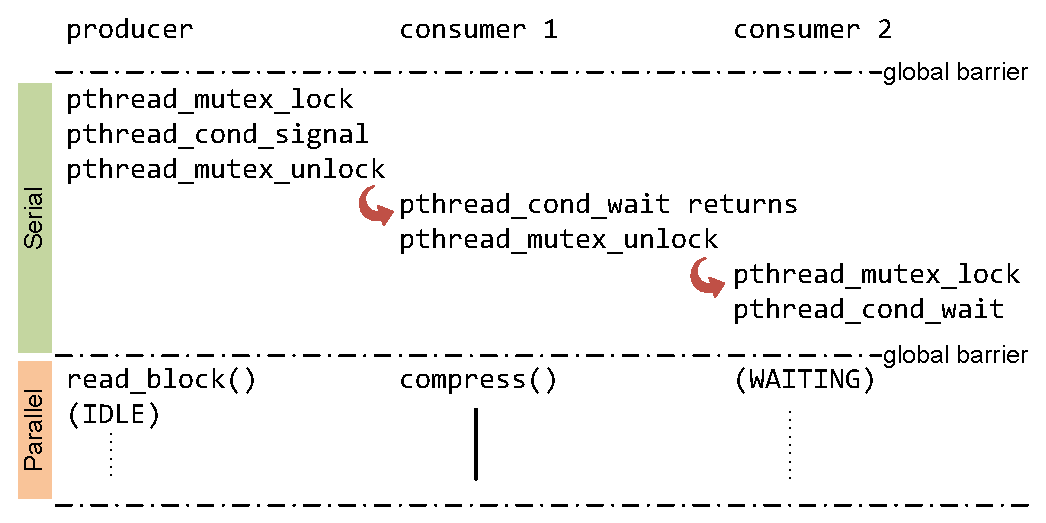
\includegraphics[width=0.6\columnwidth]{parrot/figures/dthreads_schedule}
\vspace{-.2in}
\caption{{\em A \dthreads schedule.}  All
  \v{compress} calls are serialized. \v{read\_block} runs much faster than
  \v{compress}.}\label{fig:parrot-dthreads-schedule}
\vspace{-.05in}
\end{figure}

\begin{figure}[t]
\centering
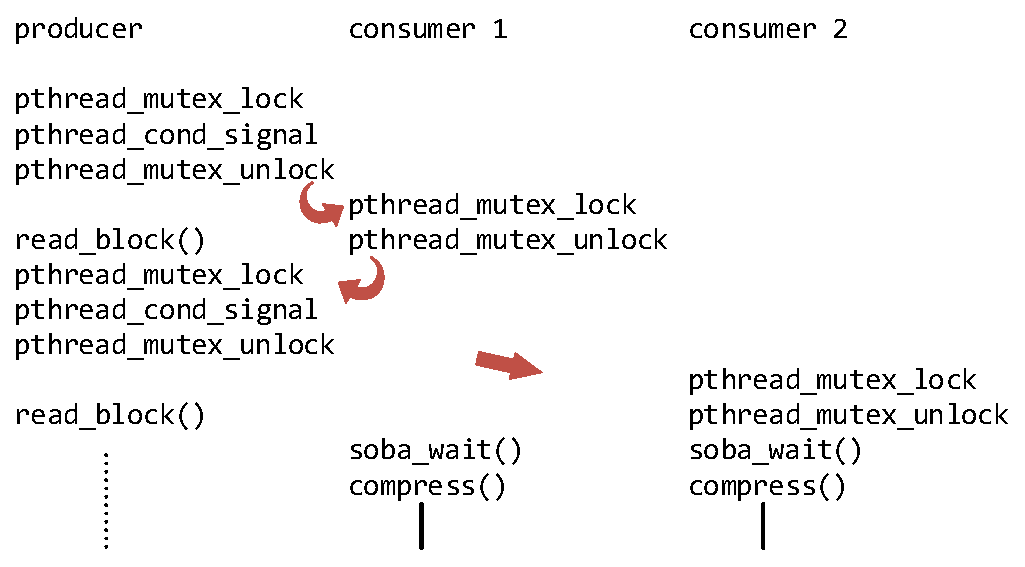
\includegraphics[width=0.6\columnwidth]{parrot/figures/parrot_schedule}
\vspace{-.2in}
\caption{{\em A \parrot schedule with performance
    hints.}}\label{fig:parrot-schedule}
\vspace{-.05in}
\end{figure}

%% In this subsection, we present an example, explain why two prior systems
%% perform poorly on it, and illustrate how \parrot works with it.

Figure~\ref{fig:parrot-example} shows the example, a simplified version of the parallel
compression utility \pbzip\cite{pbzip2}.  It uses the common producer-consumer idiom:
the producer (main) thread reads file blocks, and multiple consumer
threads compress them in parallel.  Once the number of threads and the
number of blocks are given, one synchronization schedule suffices to
compress \emph{any} file, regardless of file content or size.  Thus, this program appears
easy to make deterministic and stable.  However, previous systems suffer from
various problems doing so, illustrated below using
two representative, open-source systems.

\coredet~\cite{coredet:asplos10} represents DMT systems that balance load
by counting instructions each thread has run~\cite{coredet:asplos10,
 kendo:asplos09, dmp:asplos09, dos:osdi10, ddos:asplos13}.  While the
schedules computed may have reasonable overhead, minor input or program
changes perturb the instruction counts and subsequently the schedules,
destabilizing program behaviors.  When running the example
with \coredet on eight different files, we observed
five different synchronization schedules.  This instability is
counterintuitive and raises new reliability challenges.  For instance,
testing one input provides little assurance for very similar inputs.
Reproducing a bug may require every bit of the bug-inducing input,
including the data a user typed, environment variables, shared libraries,
\etc. Missing one bit may deterministically hide the bug.  \coredet also
relies on static analysis to detect and count shared memory load and store
instructions, but the inherent imprecision of static analysis causes it to
instrument unnecessary accesses, resulting in high overhead.  On this
example, \coredet causes a 4.2$\times$ slowdown over nondeterministic execution with a 400
MB file and 16 threads.

% \footnote{Line XXX performs the \pbzip compression functionality
% and the intput filesize $n$ is equally split for $4$ consumer threads where
% $n=4, 32, 100, 400, 800, 1k, 4k, 8k$ bytes. We condfigure \coredet 
% in ownership tracking with 64-byte granularity and a quantum 
% size of $200k$ instructions.}
%% We also observed that adding \v{printf} statements led to different
%% schedules.  This instability is counterintuitive at least, and raises new
%% reliability challenges.  For instance, testing one input provides little
%% assurance on very similar inputs.  Reproducing a bug requires every bit of
%% the bug-inducing input, including not only the data a user typed, but also
%% environment variables, shared libraries, \etc.  A single missed bit may
%% deterministically hide the bug.  We observed 4.2x slowdown over
%% nondeterministic execution with a 400 MB file and 16 threads.  The reason
%% is that \coredet statically instruments shared memory loads and stores to
%% count instructions and make data races deterministic.  However, it is a
%% known-difficult problem to statically detect which memory locations may be
%% shared, so \coredet has to conservatively instrument many loads and stores,
%% causing unnecessary overhead.

%% The performance of \coredet on this example depends on the number of threads
%% and the size of inputfile where the later one dominates.
%% By choosing a $400k$ input file with 4 threads, \coredet gives more than
%% $60\%$ overhead while $400$\v{M} file gives 3$\times$ to 4$\times$ slowdown.
%% The performance yields more than 5$\times$ slowdown when we use more than
%% 16 threads.

\dthreads~\cite{dthreads:sosp11} represents \smt systems that
ignore load imbalance among threads.  It works by
alternating between a serial and a parallel phase, separated by global
barriers.  In a serial phase, it lets each thread do one synchronization in
order.  In a parallel phase, it lets threads run until all of them are about
to do synchronizations.  A parallel phase lasts as long as the slowest
thread, and is oblivious to the execution times of the other threads.  When
running the example with two threads, we observed the \dthreads schedule
in Figure~\ref{fig:parrot-dthreads-schedule}.  This schedule is stable because it
can compress any file, but it is also very slow because it serializes all
\v{compress} calls.  We observed \dthreadsexampleoverhead slowdown
with 16 threads; and more threads give bigger slowdowns.

This \emph{serialization} problem is not specific to only
\dthreads. Rather, it is general to all \smt systems that ignore load
imbalance.

%% make
%% schedules oblivious to computations but also unrealistically assume that
%% the schedules align with computations.  It works by alternating between a
%% serial and a parallel phase, separated by global barriers.  In serial
%% phase, it lets each thread do one synchronization in order.  In parallel
%% phase, it lets threads run until all of them are about to do
%% synchronizations.  This phase lasts as long as the slowest thread, and is
%% oblivious to the execution times of the other thread.  When running the
%% example with two threads, we observed the \dthreads schedule in
%% Figure~\ref{fig:dthreads-schedule}.  This schedule is stable because it
%% can compress any file, but it is also very slow because it serializes
%% all \v{compress} calls.  We observed 7.7x slowdown with 16 threads; more
%% threads give bigger slowdowns.

%% in which threads compute
%% locally and a serial phase in which threads do synchronizations in order.
%% The phases are separated by global barriers.


%% Its schedule are thus 
%% The parallel phase lasts as long as the slowest thread
%% Its schedule is thus oblivious to the local compute time of each thread.
%% can thus process a wide range of input because it is oblivious to how long
%% each thread computes in the parallel phases.
%% However, by ignoring compute
%% time, it can also lead to serious performance overhead.  

%%  which \emph{serialized} all calls to
%% \v{compress}, yielding the slowdown proporitonal to the the number of
%% threads; 16 threads gives more than 10$\times$ slowdown.

%% \peregrine~\cite{peregrine:sosp11} represents \smt systems that make
%% schedules oblivious to computations by recording and reusing schedules.
%% Recording can be slow; we observed XXX times slowdown when running the
%% example with \peregrine.  Moreover, to reuse a schedule, \peregrine requires
%% sophisticated program analysis to compute the constraints the schedule
%% places on inputs.


Running the example with \parrot is easy; users do
\vspace{-2 mm}
\begin{small}
\begin{verbatim}
                     $ LD_PRELOAD=./parrot.so program args...
\end{verbatim}
\end{small}
\vspace{-2 mm}
% Heming: hack, added empty space to make the command exist at center place.

%, shown in Figure~\ref{fig:schedule} actually 
% more than 10 times slowdown when the number of threads is more than 16.

\noindent
During the execution, \parrot intercepts \pthread synchronizations.  Without
the hints at lines 3 and 23, \parrot schedules the synchronizations using round-robin. 
This schedule also serializes the \v{compress} calls, yielding the same slowdown as \dthreads.
Developers can easily detect this performance problem with
sample runs, and \parrot simplifies performance debugging by
deterministically reproducing the problem and reporting synchronizations
excessively delayed  by round-robin
(\eg, the return of \v{pthread\_cond\_wait} here).
%  When running the examplewith \parrot on a 400 MB file, we frequently
%  observed over 4s round-robin delay on \v{pthread\_mutex\_lock} in the
%  main thread.

To solve the serialization problem, we added a \compute at lines 3 and 23.  Line 3
informs \parrot that the program has a coscheduling group involving
\v{nthreads} threads, and line 23 is the starting point of coscheduling.  With
these hints, \parrot switched to the schedule in
Figure~\ref{fig:parrot-schedule} which ran \v{compress} in parallel,
achieving 0.8\% overhead compared to nondeterministic execution. A soft barrier is
different from classic synchronizations and can be safely 
ignored without affecting correctness.  For
instance, if the file blocks cannot be evenly divided among
the threads, the soft barrier will time out on the last round of input blocks.  Moreover,
for reasonable performance, we need to align only time-consuming computations
(\eg, \v{compress}, not \v{read\_block}).

%% Note that these hints need not be 100\% accurate because \parrot can time out
%% them without losing determinism.  Moreover, these hints need not align the
%% computation perfectly for reasonable performance.

% lasts longer than 4 seconds
%% Once developers discover this serialization, they can add \compute hints
%% (lines XX and XX) to let \parrot switch to a faster schedule that makes
%% \v{compress} calls run in parallel. In our sample run, the wait time of
%% \v{pthread\_mutex\_lock} in main thread lasts longer than 4 seconds when
%% the input file size is 400MB, which indicates a serializtion problem only
%% utilizes one thread and starves the rest.  Lines XXX and XXX show the
%% hints. Line XXX informs \parrot the size of the parallel computation group.
%% Line XXX informs \parrot the beginning point of a computation.  With the
%% hints, \parrot achieved comparable performance ($<$1\% overhead) to
%% nondeterministic execution.

%% To further help developers, \parrot also logs the wait
%% time of each synchronization for developers to identify excessive delays.

\begin{figure}[t]
\centering
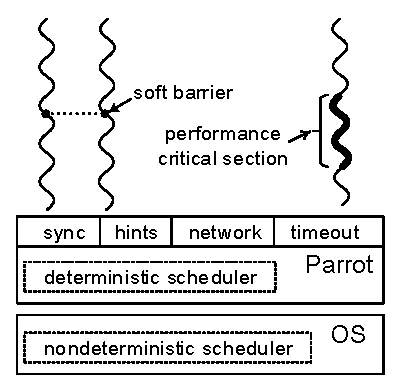
\includegraphics[width=.28\textwidth]{parrot/figures/architect}
%arch:
%programs with threads
%  computation  nondet regions
%      \  /
%       \/
%sync, hints, network, timeout, 
%deterministic scheduler, 
%OS schedule
\vspace{-.05in}
\caption{{\em \parrot architecture.}} \label{fig:parrot-arch}
\vspace{-.05in}
\end{figure}

\subsection{Architecture} \label{sec:parrot-arch}

Figure~\ref{fig:parrot-arch} shows \parrot's architecture.  We designed \parrot to be
simple and deployable.  It consists of a deterministic user-space
scheduler, implementation of hints, a set of wrapper functions for
intercepting \pthread, network, and timeout operations.  For simplicity,
the scheduler schedules only synchronizations, and delegates everything
else, such as assigning threads to CPU cores, to the OS scheduler.
The wrapper functions typically call into the scheduler for round-robin scheduling,
then delegate the actual implementation to \pthread or the OS.
Synchronizations in performance critical sections and inherently
nondeterministic operations (\eg, \v{recv}) are scheduled by the OS
scheduler.

\section{Performance Hint Abstractions} \label{sec:parrot-hints}

\parrot provides two performance-hint abstractions: a \emph{soft barrier} and
a \emph{performance critical section}.  This section describes these abstractions and
their usage.


\subsection{Soft Barrier} \label{sec:soft-barrier}

A \vcompute encourages the scheduler to coschedule a group of threads at
given program points.  It is for performance only, and a scheduler can
ignore it without affecting correctness.  It operates as a
barrier with deterministic timeouts in \parrot, helping \parrot switch to faster
schedules that avoid serializing parallel computations.  The interface is
\vspace{-3 mm}
\lgrindfile{parrot/code/compute.cpp}
\vspace{-1 mm}

\noindent
One thread calls \v{soba\_init(N, key, timeout)} to initialize the barrier
named \v{key}, logically indicating that a group of \v{N} threads will
be spawned.  Subsequently, any thread which calls \v{soba\_wait(key)}
will block until either (1) \v{N}-1 other threads have also called
\v{soba\_wait(key)} or (2) \v{timeout} time has elapsed since the first
thread arrived at the barrier.  This timeout is made deterministic by \parrot
(\S\ref{sec:parrot-scheduler}).  \v{soba\_init} can be called multiple
times: if the number of coscheduled threads varies but is known at runtime,
the soft barrier can be initialized before each use.  Both \v{key} and
\v{timeout} in \v{soba\_init} are optional.  An absent \v{key} refers to a
unique anonymous barrier.  An absent \v{timeout} initializes the barrier
with the default timeout.

A \compute may help developers express coscheduling intent to classic
nondeterministic schedulers~\cite{coschedule}.  One advantage is that it
makes the group of threads and program points explicit.  It is more robust
to developer mistakes than a real barrier~\cite{coschedule:sigmetrics96}
for coscheduling purposes because schedulers cannot ignore a real barrier.


\subsection{Performance Critical Section} \label{sec:parrot-performance-critical-section}

A \vnondet identifies a code region as a potential bottleneck
and encourages the scheduler to get
through the region fast.  When a thread enters a performance critical
section, \parrot removes the thread from the round-robin scheduling 
and delegates it to the OS scheduler for nondeterministic execution.  \parrot thus gains speed
from allowing additional schedules.  The interface is
\vspace{-3 mm}

\lgrindfile{parrot/code/nondet.cpp}
\vspace{-1 mm}

\noindent
The \v{pcs\_enter} function marks the entry of a performance critical section and
\v{pcs\_exit} the exit.

\subsection{Usage of the Two Hints} \label{sec:parrot-hints-usage}

\para{Soft barrier.} Developers should generally use soft barriers to align
high-level, time-consuming parallel computations, such as the \v{compress}
calls in \pbzip. A generic method is to use performance debugging tools or
\parrot's logs to detect synchronizations excessively delayed by \parrot's
round-robin scheduling, then identify the serialized parallel computations.

A second method is to add soft barriers based on parallel computation
patterns.  Below we describe how to do so based on four parallel
computation patterns we observed from the \nprog evaluated programs.

\begin{enumerate}

\item[$\bullet$] {\em Data partition}. Data is partitioned among worker
  threads, and each worker thread computes on a partition. This pattern is
  the most common; \ndatapartition out of the \nprog programs follow this
  pattern, including the programs with fork-join parallelism.  Most
  programs with this pattern need no soft barriers.  In rare cases when
  soft barriers are needed, developers can add \v{soba\_wait} before each
  worker's computation.  These soft barriers often work extremely well.

\item[$\bullet$] {\em Pipeline}. The threads are split into stages of a
  pipeline, and each item in the workload flows through the pipeline
  stages.  \ferret, \dedup, \vips, and \xtwosixfour from \parsec~\cite{parsec} follow this pattern.
  These programs often need soft barriers because
  threads have different roles and thus do different synchronizations,
  causing default schedules to serialize computations.  The
  methodology is to align the most time-consuming stages of the
  pipeline.

\item[$\bullet$] {\em Map-reduce}. Programs with this pattern use both data
  partition and pipeline, so the methodology follows both: align the
  map function and, if the reduce function runs for roughly the same
  amount of time as the map function, align reduce with map.

\item[$\bullet$] {\em Workpile}. The workload consists of a pile of independent
  work items, processed by worker threads running in parallel.  Among the
  programs we evaluated, \bdb, \openldap, \redis, \pfscan, and \aget fall
  in this category.  These programs often need no soft barriers because
  it typically takes similar times to process most items.

\end{enumerate}


\para{Performance critical section.} Unlike a soft barrier, a \nondet may trade
some determinism for performance. Consequently, it should be applied with caution,
only when (1) a code region imposes high performance overhead on deterministic execution
and (2) the additional schedules have been thoroughly checked by tools or
advanced developers.  Fortunately, both conditions are often easy to meet
because the synchronizations causing high performance overhead are often low-level
synchronizations (\eg, lock operations protecting a shared counter),
straightforward to analyze with local reasoning or model checkers.

Of all \nprog evaluated programs, only \nprognondethints need performance critical
sections for reasonable performance; all other \nprognonondethints
programs need not trade determinism for performance.
Moreover, \ecosys verified all schedules in all 4 real-world programs that
need performance critical sections, providing high assurance.

Developers can identify where to add performance critical sections also
using performance debugging tools.  For instance, frequent
synchronizations with medium round-robin delays are often good candidates for
a performance critical section.  Developers can also focus on such
patterns as synchronizations in a tight loop,
synchronizations inside an abstraction boundary (\eg, \v{lock()}
inside a custom memory allocator), and tiny critical sections (\eg,
``\v{lock(); x++; unlock();}'').  

%% A dominant pattern is to mark a tight loop with synchronizations as a
%% performance critical section, so \parrot can pass a thread running in the
%% loop to the OS scheduler for quick finish.

%% \nondet hints are added to tell the \parrot runtime to ignore 
%% some sync operations in perfomance critical 
%% sections, and the per-thread computation in these programs 
%% and not roughly the same (so \compute hints are not 
%% suitable for these cases). 

%% usage: low-level

%% experience: 

%% Nondeterminism hints revert back to nondeterministic execution for
%% carefully chosen code regions.  These regions are often already ``hot''
%% during nondeterministic execution by doing many synchronizations at a high
%% rate, so they cause even very high overhead when executed
%% deterministically.  By moving threads in nondeterministic regions from the
%% round-robin scheduler to the OS's scheduler, \parrot gains speed.


%% \v{nondet(var)} marks all synchronizations on synchronization variable
%% \v{var} as nondeterministic, so \parrot excludes the synchronizations from
%% its round-robin scheduling. Frequently a code region executes many
%% synchronizations touching several synchronization variables, and
%% developers can use

%% \parrot treats \v{nondet\_begin} as a special synchronization that
%% participates in round-robin scheduling, so that a nondeterministic region
%% always begins execution deterministically.  However, \parrot does not know
%% how long the region may run, so it has to let the region end
%% nondeterministically.  After the thread calls \v{nondet\_end}, \parrot adds
%% the thread back to the round-robin scheduling.

%% \para{Usage.} Unlike \compute hints, \nondet hints may trade off 
%% an amount of determinism for performance, so it should be applied with
%% caution, only when (1) a code region has high overhead on deterministic
%% execution and (2) the additional schedules have been thoroughly checked by
%% tools or advanced developers inspecting the code region.  Fortunately,
%% both conditions are often easy to meet because the synchronizations
%% causing high overhead tend to be frequent, low-level synchronizations,
%% easy to analyze with local reasoning. Among all programs 
%% we have evaluated, four real applications \pfscan, three STL programs 
%% \partition, \nthelement, and \partialsort, and five 
%% benchmark programs \fluidanimate, \fmm, 
%% \cholesky, \raytrace from \splashx, and \ua and all fall into this category.
%% For all the four real applications, our ecosystem can 
%% effectively check all these schedules in the \nondet region 
%% within a few hours. For all the five benchmarks programs, 
%% although our ecosystem can not check all their schedules in 
%% \nondet regions within one day's run, we still considered 
%% these results promising because people normally care 
%% about the correctness of real applications over benchmark 
%% programs.

%% Heming: we do not prefer to mention this because this 
%% pattern is not that common in our non-det programs. Only 
%% pfscan and fluidanimate do this.
%% A common pattern we observed on the
%% programs we evaluated is when the program uses a tiny critical section to
%% increment or decrement a shared counter.  It easy to determine based on
%% purely local reasoning that The executions of these critical section are
%% commutable.  This pattern appears in 6 out of 9 programs with \nondet
%% hints.



\section{\parrot Runtime} \label{sec:parrot-runtime}

%% The simple \parrot runtime consists of a user-space scheduler
%% (\S\ref{sec:scheduler}), a set of wrapper functions for intercepting
%% \pthread synchronizations (\S\ref{sec:sync}), implementations of the hint
%% abstractions (\S\ref{sec:hints-impl}), handlers for network operations
%% (\S\ref{sec:network}), and handlers of timeouts (\S\ref{sec:timeout}).

The \parrot runtime contains implementation of the hint abstractions
(\S\ref{sec:parrot-hints-impl}) and a set of wrapper functions that intercept
\pthread (\S\ref{sec:parrot-sync}), network (\S\ref{sec:parrot-network}), and timeout
(\S\ref{sec:parrot-timeout}) operations.  The wrappers interpose dynamically
loaded library calls via \v{LD\_PRELOAD} and ``trap'' the calls into
\parrot's deterministic scheduler (\S\ref{sec:parrot-scheduler}).  Instead of
reimplementing the operations from scratch, these wrappers leverage
existing runtimes, greatly simplifying \parrot's implementation, deployment,
and inter-operation with code that assumes standard runtimes (\eg,
debuggers).

\subsection{Scheduler} \label{sec:parrot-scheduler}

The scheduler intercepts synchronization calls and releases threads using the
well-understood, deterministic round-robin algorithm: the first thread
enters synchronization first, the second thread second, ..., and
repeat.  It does not control non-synchronization code, often the majority
of code, which runs in parallel.  It maintains a queue
of runnable threads (\emph{run queue}) and another queue of waiting
threads (\emph{wait queue}), like typical schedulers.  Only the head of the
run queue may enter synchronization next. Once the synchronization call is
executed, \parrot updates the queues accordingly.  For instance, for
\v{pthread\_create}, \parrot appends the new thread to the tail of
the run queue and rotates the head to the tail.  By maintaining
its own queues, \parrot avoids nondeterminism in the OS scheduler and
the \pthread library.

\begin{table}[t]
\centering
\small
\begin{minipage}[t]{.25\textwidth}
\lgrindfile{parrot/code/scheduler.cpp}
\end{minipage}
%% \begin{tabular}{l}
%% \v{void get\_turn(void)} \\
%% \v{void put\_turn(void)} \\
%% \v{int wait(void *addr, int timeout)} \\
%% \v{void signal(void *addr)} \\
%% \v{void broadcast(void *addr)} \\
%% \v{void block()} \\
%% \v{void wakeup()} \\
%% \end{tabular}
\vspace{-.05in}
\caption{{\em Scheduler primitives.}} \label{tab:parrot-scheduler}
\vspace{-.05in}
\end{table}

To implement operations in the \parrot runtime, the scheduler provides a
monitor-like internal interface, shown in Table~\ref{tab:parrot-scheduler}.  The
first five functions map one-to-one to functions of a typical monitor,
except the scheduler functions are deterministic.  The last two are for
selectively reverting to nondeterministic execution.  The rest of this
subsection describes these functions.

The
\v{get\_turn} function waits until the calling thread becomes the head
of the run queue, \ie, the thread gets a ``turn'' to do a
synchronization.  The \v{put\_turn} function rotates the calling thread
from the head to the tail of the run queue, \ie, the thread gives up a
turn. The \v{wait} function is similar to
\v{pthread\_cond\_timedwait}.  It requires that the calling thread has the
turn.  It records the address the thread is waiting for and the timeout
(see next paragraph), and moves the calling thread to the tail
of the wait queue.  The thread is moved to the tail of the
run queue when (1) another thread wakes it up via \v{signal}
or \v{broadcast} or (2) the timeout has expired. The \v{wait}
function returns when the calling thread gets a turn again.  Its return
value indicates how the thread was woken up. The \v{signal(void *addr)}
function appends the first thread waiting for \v{addr} to the run queue.  The
\v{broadcast(void *addr)} function appends all threads waiting for
\v{addr} to the run queue in order.  Both \v{signal} and \v{broadcast} require
the turn.

%% The \v{get\_turn()} function waits until the calling thread
%% becomes the head of the run queue, \ie, the thread gets the ``turn'' to do a
%% synchronization. The \v{put\_turn()} function rotates the calling thread from the head
%% to the tail of run queue, \ie, the thread gives up the turn. The \v{wait(void
%%   *addr, int timeout)} function is similar to \v{pthread\_cond\_timedwait}.  It
%% requires that the calling thread has the turn.  It records the address the
%% thread is waiting for and the timeout (\cf next paragraph) of the wait, and
%% moves the calling thread to the tail of the wait queue.  The thread is woken
%% up and moved to the tail of the run queue when (1) another thread wakes it up
%% via the \v{signal} function or the \v{broadcast} function or (2) the timeout has 
%% expired. The \v{wait} function returns when the calling thread gets the turn again.  Its return value
%% indicates how the thread is woken up. The \v{signal(void *addr)} function searches
%% wait queue for the first thread waiting for \v{addr} and appends it to run
%% queue. The \v{broadcast(void *addr)} function wakes up all threads waiting for \v{addr}
%% and appends them to run queue in order.  Both the \v{signal} 
%% and the \v{broadcast} functions require the turn.

The \v{timeout} in the \v{wait} function does not specify real time, but relative \emph{logical time} that
counts the number of turns executed since the beginning of current
execution.  In each call to the \v{get\_turn} function, \parrot increments this logical
time and checks for timeouts. 
(If all threads block, \parrot keeps the logic time advancing with an idle
thread; see~\S\ref{sec:parrot-timeout}.)
The \v{wait} function takes a relative timeout argument.  If
current logical time is $t_l$, a timeout of 10 means waking up the thread
at logical time $t_l + 10$. A \v{wait(NULL, timeout)} 
call is a logical sleep, and a \v{wait(addr, 0)} call never times out.
% Logical time makes it easy to implement many operations real-world
% programs rely on (\S\ref{sec:timeout}).

\begin{figure}[t]
\centering
\begin{minipage}[t]{.38\textwidth}
\lgrindfile{parrot/code/lock.cpp}
\end{minipage}
\vspace{-1 mm}
\caption{{\em Wrappers of \pthread mutex lock\&unlock.}} \label{fig:parrot-lock}
\vspace{-0.0in}
\end{figure}

The last two functions in Table~\ref{tab:parrot-scheduler} support performance
critical sections and network operations.  They set the calling thread's
execution mode to nondeterministic or deterministic. \parrot always schedules
synchronizations of deterministic threads using round-robin, but it lets
the OS scheduler schedule nondeterministic threads.
Implementation-wise, the \v{nondet\_begin} function marks the calling
thread as nondeterministic and simply returns.  This thread will be lazily
removed from the run queue by the thread that next tries to pass the turn to it.
(Next paragraph explains why the lazy update.)
The \v{nondet\_end} function marks the calling thread as deterministic and
appends it to an additional queue.  This thread will be lazily appended to
the run queue by the next thread getting the turn.

We have optimized the multicore scheduler implementation for the most frequent
operations: \v{get\_turn}, \v{put\_turn}, \v{wait}, and \v{signal}.  Each
thread has an integer flag and condition variable. The \v{get\_turn} function
spin-waits on the current thread's flag for a while before block-waiting
on the condition variable. The \v{wait} function needs to get the turn before it
returns, so it uses the same combined spin- and block-wait strategy as
the \v{get\_turn} function. The \v{put\_turn} and the 
\v{signal} functions signal both the flag and the
condition variable of the next thread.  In the common case, these
operations acquire no lock and do not block-wait.  The lazy updates above
simplify the implementation of this optimization by maintaining the
invariant that only the head of the run queue can modify the run and wait
queues.

%% In order to support \nondet operations such as I/O operations, 
%% we introduce two more schedule primitives. The first one is 
%% \v{block()} called by a thread before doing a \nondet 
%% operation. It gets turn, removes it self from \emph{run queue}, 
%% and then passes the turn to the thread in the head of the \emph{run queue}. 
%% This operation ensures that  while a thread is doing a \nondet operation,
%% it self is not in the \emph{run queue} of \parrot, so that the \parrot runtime 
%% does not enforce any order between it and other threads within the runtime 
%%  (deadlock-free). The second one \v{wakeup()} is called 
%%  after a thread gets back from a \nondet opeartion. It appends the thread 
%%  itself to a \emph{wakeup queue} , an extra data structure for \nondet 
%%  operations. In \parrot, after each thread gets its turn, it  will check this 
%%  \emph{wakeup queue} and put the threads from this queue back to
%%  \emph{runq queue}. A thread getting back from \nondet operations to
%% \parrot runtme is not allowed to put itself back to the \emph{runq 
%% queue}  directly, because our \parrot runtime ensures that only the 
%% head of \emph{runq queue} is allowed to modify the \emph{runq queue}.

\subsection{Synchronizations} \label{sec:parrot-sync}

%% The wrapper functions intercept \pthread synchronizations by interposing
%% dynamically loaded library calls (via \v{LD\_PRELOAD}) and ``trapping''
%% them into the scheduler.  Wrappers are simple.  Instead of reimplementing
%% \pthread synchronizations from scratch, they leverage existing \pthread
%% runtimes, greatly simplifying the code, deployment, and inter-operation
%% with code that assumes standard \pthread runtimes (\eg, debuggers).
% Wrappers replicate a small amount of control data in the \pthread
% runtime, such as the size of a barrier and the locked status of a mutex,
% to determine whether the intercepted synchronizations block.
%% Wrappers ensure a total (round-robin) order of synchronizations by (1)
%% using the scheduler primitives to ensure that at most one wrapper has the
%% turn and (2) executing the actual synchronizations only when the turn is held.

% To do so, the first thing a wrapper does is to wait for its turn, \ie,
% the calling thread becoming the head of the queue, and the last thing is
% to give up the turn by moving the calling thread to the tail of the run
% or wait queue.

\parrot handles all synchronizations on \pthread mutexes, read-write
locks, condition variables, semaphores, and barriers. It also handles thread
creation, join, and exit.  It need not implement the other \pthread
functions such as thread ID operations, another advantage of leveraging
existing \pthread runtimes. In total, \parrot has \npthreadsync synchronization
wrappers.  They ensure a total (round-robin) order of synchronizations by
(1) using the scheduler primitives to ensure that at most one wrapper has
the turn and (2) executing the actual synchronizations only when the turn
is held.

%  Below we illustrate how we implemented the \parrot runtime for three example synchronizations.
% (Interested readers may refer to \parrot's source code~\cite{parrot-github}
% for others.)

% \subsubsection{Locks}

Figure~\ref{fig:parrot-lock} shows the pseudo code of our \pthread mutex lock and
unlock wrappers.  Both are quite simple; so are most other wrappers.  The
lock wrapper uses the try-version of the \pthread lock operation to avoid
deadlock: if the head of run queue is blocked waiting for a lock before
giving up the turn, no other thread can get the turn.

%% For \v{pthread\_mutex\_lock} but the lock is already held,
%% \parrot moves the current thread from the head of the run queue to the tail
%% of the wait queue and record the address of the mutex the thread is
%% waiting for.  For \v{pthread\_mutex\_unlock}, \parrot wakes up the first
%% thread waiting for the mutex if there is one from the wait queue.  After
%% running the synchronizations, \parrot rotates the current thread to the end
%% of the run queue if the synchronization did not cause it to block on the
%% wait queue.  

%% The unlock wrapper.

% \subsubsection{Condition Variables} \label{sec:cond_wait}

\begin{figure}[t]
\centering
\begin{minipage}[t]{.5\textwidth}
\lgrindfile{parrot/code/cv.cpp}
\end{minipage}
\vspace{-2 mm}
\caption{{\em Wrapper of \v{pthread\_cond\_wait}.}} \label{fig:parrot-cv}
\vspace{-0 mm}
\end{figure}

Figure~\ref{fig:parrot-cv} shows the \v{pthread\_cond\_wait}
wrapper.  It is slightly more complex than the lock and unlock wrappers
for two reasons.  First, there is no try-version of
\v{pthread\_cond\_wait}, so \parrot cannot use the same trick to avoid
deadlock as in the lock wrapper.  Second, \parrot must ensure that unlocking
the
mutex and waiting on the conditional variable are atomic (to avoid the
well-known lost-wakeup problem).  \parrot solves these issues by implementing
the wait with the scheduler's \v{wait} which atomically gives up the
turn and blocks the calling thread on the wait queue.  The wrapper of
\v{pthread\_cond\_signal} (not shown) calls the scheduler's \v{signal}
accordingly.

%% which blocks the calling thread regardless, \parrot must release the
%% scheduler lock before the blocking to avoid deadlock.  Yet, if \parrot lets
%% the synchronization run outside of

%% \subsubsection{Thread Creation}

%% \begin{figure}[t]
%% \centering
%% \begin{minipage}[t]{.5\textwidth}
%% \lgrindfile{code/pthread_create.cpp}
%% \end{minipage}
%% \caption{{\em Wrapper of \v{pthread\_create}.}} \label{fig:create}
%% \end{figure}

%% \begin{figure}[t]
%% \begin{verbatim}
%% two threads calling pthread_create, two new threads
%% first pthread\_create thread wrongly pairs up
%%    with last new thread
%% \end{verbatim}
%% \caption{{\em \v{pthread\_create} race.}} \label{fig:create-race}
%% \end{figure}

% Figure~\ref{fig:create} shows the pseudo code of the \v{pthread\_create}
% wrapper.

Thread creation is the most complex of all wrappers for two reasons.
First, it must deterministically assign a logical thread ID
to the newly created thread because the system's thread IDs are
nondeterministic.  Second, it must also prevent the new thread from using
the logical ID before the ID is assigned.  \parrot solves these issues by
synchronizing the current and new threads with two semaphores, one to make
the new thread wait for the current thread to assign an ID, and the other to
make the current thread wait until the child gets the ID.

%% Specifically, \v{wrap\_thread\_create} waits for the turn, saves the
%% user-provided thread function, and calls the actual \v{pthread\_create} to
%% create a thread to run \v{wrap\_thread\_func}, a wrapper to the
%% user-provided thread function.  Function \v{wrap\_thread\_create}
%% continues by recording the mapping from the new thread's \pthread ID to
%% logical thread ID, and adds the new thread to run queue.  It then
%% wakes up the new thread blocked inside \v{wrap\_thread\_func}, waits for
%% the new thread to get its logical thread ID, and finally gives up the
%% turn.  Both semaphores are necessary.  Function \v{wrap\_thread\_func}
%% must wait for \v{wrap\_thread\_create} to set up the mapping from the
%% \pthread ID to logical ID.  Function \v{wrap\_thread\_create} must wait for
%% \v{wrap\_thread\_func} before giving the turn because otherwise another
%% newly created thread may be wrongly woken up.
%, as illustrated in Figure~\ref{fig:create-race}.

%% One complication is the wrapper of \v{pthread\_cond\_wait(cond, mutex)}.
%% This synchronization blocks the calling thread on condition variable
%% \v{cond} regardless, so \parrot must release the scheduler lock before the
%% blocking to avoid deadlock.  However, the semantics also requires that
%% unlocking \v{mutex} and waiting on \v{cond} be atomic (to avoid the
%% lost-wakeup problem).

\subsection{Performance Hints} \label{sec:parrot-hints-impl}

%% \begin{figure}[t]
%% \centering
%% \begin{minipage}[t]{.5\textwidth}
%% \lgrindfile{code/compute-algo.cpp}
%% \end{minipage}
%% \caption{{\em Pseudo code of soft barrier.}} \label{fig:compute}
%% \end{figure}

%% Figure~\ref{fig:compute} shows the implementation of soft barrier, a
%% reusable barrier with a deterministic timeout.  \parrot implements

\parrot implements performance hints using the scheduler primitives.  It
implements the soft barrier as a reusable barrier with a deterministic
timeout.  It implements the performance critical section by simply calling
\v{nondet\_begin()} and \v{nondet\_end()}.
% to temporarily enable nondeterministic execution of a thread within a
% performance critical region.

One tricky issue is that deterministic and nondeterministic executions may
interfere.  Consider a deterministic thread $t_1$ trying to lock a mutex
that a nondeterministic $t_2$ is trying to unlock.
Nondeterministic thread $t_2$ always ``wins'' because the timing of
$t_2$'s unlock directly influences $t_1$'s lock regardless of how hard
\parrot tries to run $t_1$ deterministically.  An additional concern is
deadlock: \parrot may move $t_1$ to the wait queue but never wake $t_1$ up
because it cannot see  $t_2$'s unlock.

To avoid the above interference, \parrot requires that synchronization variables accessed
in nondeterministic execution are isolated from those accessed in
deterministic execution.  This \emph{strong isolation} is easy to achieve based
on our experiments because, as discussed in~$\S$\ref{sec:parrot-hints}, the
synchronizations causing high overhead on deterministic execution tend to
be low-level synchronizations already isolated from other
synchronizations. To help developers write performance critical sections
that conform to strong isolation, \parrot checks this property at runtime:
it tracks two sets of synchronization variables accessed within
deterministic and nondeterministic executions, and emits a warning when the
two sets overlap.  Strong isolation is considerably stronger than
necessary: to avoid interference, it suffices to forbid
deterministic and nondeterministic sections from \emph{concurrently}
accessing the same synchronization variables.  We have not implemented
this \emph{weak isolation} because strong isolation works well for all
programs evaluated.

%%  before each \nondet operation.  Although this
%% approach is crude, we find it pretty lightweight and the warnings are
%% already quite helpful to us when adding \nondet hints.

%% One concern with our implementation of \nondet hints is deadlock.  The
%% system scheduler runs all threads in nondeterministic regions, whereas
%% \parrot runs all other threads.  The system scheduler and \parrot may attempt to
%% enforce contradictory constraints, causing deadlocks like in
%% Figure~\ref{fig:deadlock}.

%% We sketch a proof that our implementation of performance critical section
%% does not introduce deadlocks.  Suppose a program has no deadlock running
%% with either the system's scheduler or \parrot, but it has a deadlock when
%% running with both.  There are two scenarios.  First, the head of run queue
%% is blocked without giving up the turn. The blocking synchronization must
%% be done by a nondeterministic thread, or \parrot would have noticed.
%% However, this scenario is impossible because a nondeterministic thread
%% cannot be the head of run queue.  Second, some thread on wait queue should
%% have been signaled but was not.  The lost signal must be done by a
%% nondeterministic thread, but this scenario is also impossible because
%% synchronization variables are strongly isolated.


%% The \compute hint works in a similar way as \pthread 
%% barrier, except it has a deterministic logical timeout. 
%% When a thread fires a timeout for this hint, all the other 
%% threads blocking on this hint will be waken up, get turn and then proceed.
%% This deterministic logical timeout ensures that \compute 
%% hint does not affect the correctness of a program and the 
%% execution is still deterministic.

%% The \v{nondet\_begin()} hint removes the current thread from \emph{run 
%% queue}, and let the system scheduler run it. When the 
%% threa gets back, the \v{nondet\_end()} hint add it self 
%% back to the \emph{wakeup queue}, and the next thread 
%% getting the turn will put all threads from \emph{wakeup 
%% queue} back to \emph{run queue}. The system scheduler schedules 
%% all threads in nondet region.  \parrot schedulers all other threads.

%% Mixing deterministic and nondeterministic executions is tricky because
%% they can interfere.  Consider two threads: $t_1$ in deterministic
%% execution trying to lock a mutex and $t_2$ in nondeterministic execution
%% trying to unlock the same mutex.  The nondeterministic thread $t_2$ always
%% ``wins'' because regardless of how hard \parrot tries to run $t_1$
%% deterministically, the timing of $t_2$'s unlock directly influences
%% $t_1$'s lock.  In general, each nondeterministic synchronization may
%% interfere with deterministic execution.  As nondeterministic
%% synchronizations accumulate, their effects cascade boundlessly, ruining
%% deterministic execution.  Worse, since a code region may execute many
%% synchronizations, a single pair of \v{nodet\_begin} and \v{nondet\_end}
%% may have a drastic effect on determinism, extremely counterintuitive to
%% developers.

%% To avoid interference, we have carefully designed the semantics of \nondet
%% hints to strongly isolate synchronization variables accessed in
%% nondeterministic execution from those accessed in deterministic execution,
%% which \parrot checks at run time (\S\ref{sec:hints-impl}).  This strong
%% isolation turned out to be pretty easy to achieve on the programs we
%% evaluated because the synchronizations causing high overhead on
%% deterministic execution tend to be frequent, low-level synchronizations
%% that are already isolated from other synchronizations (\eg,
%% synchronizations protecting the increment of a shared counter).

%% Strong isolation has three nice features.  First, it bounds the effects of
%% the execution of a nondeterministic region on deterministic
%% execution---regardless of how many synchronizations are run, the only
%% effect is the nondeterministic execution ending.  Second, it vastly
%% simplifies the implementation of \nondet hints, to the extent that we
%% proved that our implementation is deadlock-free (\S\ref{sec:hints-impl}).
%% Third, it greatly reduces the number of executions a model checker has to
%% check because the nondeterministic synchronizations do not affect
%% deterministic executions.

%% In order to assist users to ensure strong isolation of synchronization
%% variables accessed in deterministic and nondeterministic 
%% regions, \parrot simply tracks the variables during their life time with two sets.
%% For each synchronization, it adds the variable to the
%% corresponding set protected by an internal spin lock. \parrot emits warnings
%% when the two sets overlap before each \nondet operation.
%% Although this approach is crude, we find it pretty lightweight
%% and the warnings are already quite helpful to us when adding \nondet hints.

%% One concern with our implementation of \nondet hints is deadlock.  The
%% system scheduler runs all threads in nondeterministic regions, whereas
%% \parrot runs all other threads.  The system scheduler and \parrot may attempt to
%% enforce contradictory constraints, causing deadlocks like in
%% Figure~\ref{fig:deadlock}.

%% We present a proof sketch that our \nondet hints do not introduce
%% deadlocks.  Suppose a program has no deadlock running with either the
%% system's scheduler or \parrot, but it has a deadlock when running with both.
%% There are two scenarios.  First, the head of the queue is blocked without
%% giving up the turn. The blocking synchronization must be inside a
%% nondeterministic region, like XXX in Figure~\ref{fig:deadlock}, or \parrot
%% would have noticed.  However, this scenario is impossible because a thread
%% running in a nondeterministic region is removed from \parrot's run queue and
%% cannot be the head of the queue.  Second, some thread on \parrot's wait queue
%% should have been signaled but was not.  The lost signal must be inside a
%% nondeterministic region, but this scenario is also impossible because
%% synchronization variables are strongly isolated.

%% We present a proof sketch that our \nondet hints do not introduce
%% deadlocks.  Suppose a program has no deadlock running with either the
%% system's scheduler or \parrot, but it has a deadlock when running with both.
%% Consider the \emph{wait cycle} of the deadlock, a graph with
%% synchronizations as vertexes and edges from synchronization $s_1$ to $s_2$
%% if $s_1$ can run only after $s_2$.  Figure~\ref{fig:deadlock} is an
%% example.  We use dotted lines to indicate the edges enforced by \parrot for
%% round-robin, and solid lines for those due to synchronization semantics.
%% The wait cycle of the deadlock must involve at least one synchronization
%% blocked by \parrot for round-robin and another blocked by the system's
%% scheduler due to synchronization semantics.  (Otherwise, the program has a
%% deadlock with either the system's scheduler or \parrot.)  The path from the
%% latter synchronization to the former in the wait cycle must have an edge
%% from a synchronization to a deterministic one.  Due to strong isolation,
%% these two synchronizations must be in the same thread, like XX and XX in
%% Figure~\ref{fig:deadlock}.  However, this edge is impossible because a
%% thread running in a nondeterministic region, 

%% by the system's scheduler waiting be woken up by another
%% synchronization. Otherwise, the program has a deadlock with either the
%% system's scheduler or \parrot.  The path from the

%% one synchronization
%% blocked by \parrot for the turn and another blocked by the system's scheduler
%% waiting be woken up by another synchronization.  

\subsection{Network Operations} \label{sec:parrot-network}

To handle network operations, \parrot leverages the \v{nondet\_begin} and
\v{nondet\_end} primitives.  Before a blocking operation such as \v{recv},
it calls \v{nondet\_begin} to hand the thread to the OS scheduler.  When
the operation returns, \parrot calls \v{nondet\_end} to add the thread back to
deterministic scheduling.  \parrot supports \nioync network
operations such as \v{send}, \v{recv}, \v{accept}, and \v{epoll\_wait}.
This list suffices to run all evaluated programs that require network
operations (\bdb, \openldap, \redis, and \aget).

\subsection{Timeouts} \label{sec:parrot-timeout}

Real-world programs frequently use timeouts (\eg, \v{sleep},
\v{epoll\_wait}, and \v{pthread\_cond\_timedwait}) for periodic activities
or timed waits.  Not handling them can lead to nondeterministic execution and
deadlocks.  One deadlock example in our evaluation was running \pbzip with
\dthreads: \dthreads ignores the timeout in
\v{pthread\_cond\_timedwait}, but \pbzip sometimes relies on the timeout to finish.

\parrot makes timeouts deterministic by proportionally converting them to a
logical timeout.  When a thread registers a relative timeout that fires
$\Delta t_r$ later in real time, \parrot converts $\Delta t_r$ to a relative
logical timeout $\Delta t_r /R$ where $R$ is a configurable conversion
ratio. ($R$ defaults to 3 $\mu$s, which works for all evaluated programs.)
Proportional conversion is better than a fixed logical timeout because it
matches developer intents better (\eg, important activities
run more often).  A nice fallout is that it makes some
non-terminating executions terminate for model checking
(\S\ref{sec:parrot-coverage}).  Of course, \parrot's logical time corresponds
loosely to real time, and may be less useful for real-time applications.\footnote{
dOS~\cite{dos:osdi10} discussed the possibility of converting real time to
logical time but did not present how.}

%% \parrot makes timeouts deterministic by proportionally converting them to a
%% logical timeout.  When a thread registers a relative timeout that fires
%% $\Delta t_r$ later in real time, \parrot converts $\Delta t_r$ to a relative
%% logical timeout $\Delta t_r /R$ where $R$ is a configurable conversion
%% ratio (default is 3 $\mu$s), which worked for all evaluated programs.
%% Proportional conversion is better than a fixed logical timeout because it
%% matches developer intents better.  For instance, developers may want to
%% perform one important periodical activity with higher frequency, and a
%% less important one with lower frequency.  Proportional conversion keeps
%% the relative ratio of the frequencies, and improves performance based on
%% our experiments. A nice fallout is that it makes some non-terminating
%% executions terminate for model checking (\S\ref{sec:coverage}).
%% Of course, \parrot's logical time corresponds loosely to
%% real time, and may be less useful for real-time applications.
%% (dOS~\cite{dos:osdi10} discussed the possibility of converting real to
%% logical time but did not present how.)

When all threads are on the wait queue, \parrot spawns an idle thread to keep the
logical time flowing. The thread repeatedly gets the turn, sleeps for time
$R$, and gives up the turn.  An alternative to idling is
fast-forwarding~\cite{modist:nsdi09,dos:osdi10}.  Our experiments show
that using an idle thread has better performance than fast-forwarding
because the latter often wakes up threads prematurely before the pending
external events (\eg, receiving a network packet) are done, wasting CPU cycles.

%% Moreover, it fast-forwards logical time after all threads block, slower
%% than using an idle thread.

\parrot handles all common timed operations such as \v{sleep} and
\v{pthread\_cond\_timedwait}, enough for all five evaluated programs
that require timeouts (\pbzip, \bdb, \mplayer, \imagick, and \redis).
\pthread timed synchronizations use absolute time, so \parrot provides
developers a function \v{set\_base\_time} to pass in the base time.  It
uses the delta between the base time and the absolute time argument as $\Delta
t_r$.
% The following programs we evaluated require timeout support: .

%% We find supporting these operations crucial, because lots
%% of real applications such as \pbzip, \bdb, \mplayer, \imagick and \redis
%% use them. One main reason that we could not make \dthreads and \coredet
%% work with any real application in our benchmarks during performance
%% comparison (Figure~\ref{fig:comparison}) is they did not support these
%% operations.







\section{\parrot-\dbug Ecosystem} \label{sec:parrot-mc}

%% In this section, we present an ecosystem formed by integrating \parrot with
%% the model checker \dbug~\cite{dbug:spin11}.  We present some background and rationale
%% (\S\ref{sec:mc-background}), briefly introduce \dbug (\S\ref{sec:dbug}),
%% and describe the integration (\S\ref{sec:smt+mc}).

%% \subsection{Background and Rationale} \label{sec:mc-background}

Model checking is a formal verification technique that systematically
explores possible executions of a program for bugs.  These executions
together form a \emph{state space} graph, where states are snapshots of the
running program and edges are nondeterministic events that move the
execution from one state to another.  This state space is typically very
large, impossible to completely explore---the so-called \emph{state-space
  explosion} problem.  To mitigate this problem, researchers have created
many heuristics~\cite{yang:fisc:osdi,musuvathi:aodv,killian:macemc:nsdi07} to guide the exploration toward executions
deemed more interesting, but heuristics have a risk of missing bugs.
\emph{State-space reduction} techniques~\cite{flanagan:dynamicpo,godefroid:verisoft,demeter:sosp11} soundly prune
executions without missing bugs, but the effectiveness of these techniques
is limited.  They work by discovering equivalence: given
that execution $e_1$ is correct if and only if $e_2$ is, we need check only
one of them. Unfortunately, equivalence is rare and extremely challenging
to find, especially for \emph{implementation-level} model checkers which
check implementations directly~\cite{godefroid:verisoft,musuvathi:aodv,yang:fisc:osdi,yang:explode:osdi,killian:macemc:nsdi07,dbug:spin11}.
This difficulty is reflected in the existence of only two main reduction
techniques~\cite{flanagan:dynamicpo, demeter:sosp11} for these implementation-level model
checkers.  Moreover, as a checked system scales, the state space after
reduction still grows too large to fully explore.  Despite
decades of effort, state-space explosion remains the bane of model
checking.

As discussed in~$\S$\ref{sec:parrot-intro}, integrating \smt and model checking is
mutually beneficial.  By reducing schedules, \smt offers an extremely
simple, effective way to mitigate and sometimes completely solve the
state-space explosion problem without requiring equivalence.  For
instance, \parrot enables \dbug to verify \nprogverifiedxxx programs,
including 4 programs containing \nondets (\S\ref{sec:parrot-coverage}).
In return, model
checking helps check the schedules that matter for \parrot and developers.
For instance, it can check the default schedules chosen by \parrot, the
faster schedules developers choose using \computes, or the schedules
developers add using \nondets.

%% One interesting idea is to
%% leverage these mutual benefits to release software early with a small set
%% of tested schedules, then gradually increase the schedules for performance
%% after they have been model checked. We leave this idea to future work.

%% \smt offers an extremely simple, effective way to reduce the
%% state space by reducing many schedules.  It then enforces the checked
%% schedules at runtime, greatly increasing model checking coverage.  We call
%% this approach what-you-check-is-what-you-run.  On the flip side, model
%% checking can check the schedules that matter to \smt.

\subsection{The \dbug Model Checker} \label{sec:parrot-dbug}

In principle, \parrot can be integrated with many model checkers.  We chose
\dbug~\cite{dbug:spin11} for three reasons.  First, it is 
open source, checks implementations directly, and 
supports \pthread synchronizations and Linux 
socket calls.  Second, it implements one of the
most advanced state-space reduction techniques---dynamic partial order
reduction (DPOR)~\cite{flanagan:dynamicpo}, so the further reduction \parrot
achieves is more valuable.  Third, \dbug can estimate the size of the
state space based on the executions explored, a technique particularly
useful for estimating the reduction \parrot can achieve when
the state space explodes.

Specifically, \dbug represents the state space as an \emph{execution tree}
where nodes are states and edges are choices representing the operations
executed.  A path leading from the root to a leaf encodes a unique test
execution as a sequence of nondeterministic operations.  The total number
of such paths is the state space size.  To estimate this size based on
a set of explored paths, \dbug uses the \emph{weighted backtrack
  estimator}~\cite{Kilby2006}, an online variant of Knuth's offline
technique for tree size estimation~\cite{Knuth1975}.  It treats the set of
explored paths as a sample of all paths assuming uniform distribution over
edges, and computes the state space size as the number of explored
paths divided by the aggregated probability they are explored.

%% Formally, every time a path is
%% explored, WBE updates the estimate to:
%% \[
%% \mathit{estimate} =
%% %\frac{\sum\limits_{b \in B} p(b) * p^{-1}(b)}{\sum\limits_{b \in B} p(b)} =
%% \frac{|B|}{\sum\limits_{b \in B} p(b)}
%% \]
%% where $B$ is the set of explored paths, and $p(b)$ is the probability of
%% exploring the path. For a path $b = (v_1, \ldots, v_n)$, where $v_i$ is
%% the $i$-th node along the path $b$, the probability $p(b)$ is defined
%% as: \[\prod\limits_{i = 1}^{n - 1} \frac{1}{E(v_i)}\] where $E(v_i)$ is
%% the number of edges originating from $v_i$.

%% We have integrated \parrot with a model checker called
%% \dbug~\cite{dbug:spin11}.  We chose \dbug over other model checkers for
%% three reasons.

%% First, it runs in Linux and readily supports Pthreads.
%% Second, \dbug implements some of the most advanced state-space reduction
%% techniques such as dynamic partial order reduction~\cite{popl:dpor}, so
%% the further reduction \parrot can achieve is more valuable.  Third, \dbug
%% provides a technique to estimate the state space size based on the
%% executions explored~\cite{xxx}.  Given that model checkers often cannot
%% fully explore the state space, \dbug's estimated state space size help us
%% compute an estimated reduction \parrot can achieve.

%% \subsubsection{State Space Exploration}
\dbug~\cite{dbug:spin11} is a tool for systematic testing of concurrent
Linux programs. The goal of \dbug is to explore the state space of
different program states of a concurrent program by systematically
enumerating different orders in which concurrent POSIX threads and
Linux sockets calls can be exercised by a program test.

To this end, \dbug abstractly represents the state space of a program
test using an \emph{execution tree}. Nodes of the execution tree
represent non-deterministic choice points and edges record
non-deterministic choices representing program state transitions. A
branch leading from the root of the tree to a leaf thus encodes a
unique test execution as a sequence of non-deterministic scheduling
choices.

\dbug uses this abstraction to repeatedly execute a program test,
recording what sequence of program state transition have been explored
by each iteration and guaranteeing that different iterations explore
different sequences.

\subsubsection{State Space Reduction}
To mitigate the combinatorial explosion resulting from having to
consider all possible permutations of concurrently enabled
transitions, \dbug implements dynamic partial order
reduction (DPOR)~\cite{flanagan:dynamicpo}.

A key building block of DPOR is the \emph{independence} relation that
identifies pairs of commutitative program state transitions. To avoid
the prohibitive overhead of having to track each memory access to
compute the independence relation precisely, \dbug adopts the approach
used by RacePro~\cite{racepro:sosp11}. In particular, for each program state
transition, \dbug records what abstract resources this transition
accesses, and uses this information to approximate the independence
relation.

\subsubsection{State Space Estimation}
To estimate the progress of the exploration, \dbug uses the
\emph{weighted backtrack estimator} (WBE)~\cite{Kilby2006} to estimate
the size of a partially explored execution tree. WBE is an online
variant of Knuth's offline technique for tree size
estimation~\cite{Knuth1975}. WBE uses the length of each explored branch
weighted by the probability it is explored (assuming uniform
distribution over edges) to predict the size of the tree. Formally,
WBE updates the estimate every time a branch of the execution is
explored, setting the estimate to:
\[
\mathit{estimate} =
\frac{\sum\limits_{b \in B} p(b) * p^{-1}(b)}{\sum\limits_{b \in B} p(b)} =
\frac{|B|}{\sum\limits_{b \in B} p(b)}
\]
where $B$ is the set of explored branches, and $p(b)$ is the
probability of exploring the branch. For a branch $b = (v_1, \ldots,                                                                                          
v_n)$, where $v_i$ is the $i$-th node along the branch $b$, the
probability $p(b)$ is defined as: \[\prod\limits_{i = 1}^{n - 1}
\frac{1}{E(v_i)}\] where $E(v_i)$ is the number of enabled
edges originating from node $v_i$.

\subsubsection{Source Code Annotations}
In general, \dbug does not require any changes to the source code. In
fact, as \dbug uses run-time interposition to control the order in
which concurrent POSIX threads and Linux sockets calls happen, it does
not require access to the source code at all.  However, similar to the
SysNam annotations, in some cases, source code annotations can improve
the efficiency of \dbug.

For example, a programmer can use the {\tt \dbug\_off()} and {\tt
  \dbug\_on()} annotations to exclude parts of the tested program from
the scope of \dbug, avoiding exploration of uninteresting call
interactions. (Example: using a lock to increment a variable in
pfscan). Further, a programmer can use the {\tt int \dbug\_nondet(int
  event)} function to identify a non-deterministic event. The first
time such an event occurs, \dbug records its value and makes sure the
same value is used for the same event in future iterations. (Example:
Recording the return values of {\tt gettimeofday()} for redis).
Finally, a programmer can use the {\tt int \dbug\_choose(int n)}
function to non-determinstically choose a value between $0$ and
$n-1$. (Example: Simulating timeouts or system call failures).


\subsection{Integrating \parrot and \dbug} \label{sec:parrot-smt+mc}

A key integration challenge is that both \parrot and \dbug control the order
of nondeterministic operations and may interfere, causing
difficult-to-diagnose false positives.  A na\"{i}ve solution
is to replicate \parrot's scheduling algorithm inside \dbug.  This
approach is not only labor-intensive, but also risky because the
replicated algorithm may diverge from the real one, deviating the checked
schedules from the actual ones.

Fortunately, the integration is greatly simplified because performance
critical sections make nondeterminism explicit, and \dbug can ignore
operations that \parrot runs deterministically.  \parrot's strong-isolation
semantics further prevent interference
between \parrot and \dbug.  Our integration uses a nested-scheduler
architecture similar to Figure~\ref{fig:parrot-arch} except the
nondeterministic scheduler is \dbug.  This architecture is transparent
to \dbug, and requires only minor changes (\locsmcmc lines) to \parrot.
First, we modified \v{nondet\_begin} and \v{nondet\_end} to turn \dbug
on and off.  Second, since \dbug explores event orders only after
it has received the full set of concurrent events, we modified
\parrot to notify \dbug when a thread transitions between the run queue
and the wait queue in \parrot. These notifications help \dbug accurately
determine when all threads in the system are waiting for \dbug to make
a scheduling decision.

We found two pleasant surprises in the
integration.  First, \computes speed up \dbug executions.  Second,
\parrot's deterministic timeout (\S\ref{sec:parrot-timeout}) prevents \dbug from
possibly having to explore infinitely many schedules.  Consider the
``\v{while(!done) sleep(30);}'' loop which can normally
nondeterministically repeat any number of times before making
progress.  This code has only one schedule with \ecosys because \parrot
makes the \v{sleep} return deterministically.

%% that runs \parrot inside
%% a model checker.  \parrot deterministically schedules all synchronizations
%% outside of nondeterministic regions, so it hides them from the model
%% checker.  It exposes the events in nondeterministic regions to the model
%% checker, which can then systematically explore different orders of these
%% events.  This architecture is transparent to a model checker, enabling
%% \parrot to leverage whatever model checkers~\cite{xxx}, advanced search
%% heuristics, and state-space reduction techniques~\cite{xxx}.  It also
%% requires little change to \parrot to forward the nondeterministic events to
%% the model checker.

%% To integrate \parrot with \dbug, we made no change to \dbug and only two
%% minor changes to \parrot.  First, we modified \v{nondet\_begin} and
%% \v{nondet\_end} to attach and detach a thread to \dbug, so that \dbug can
%% track the events executed in nondeterministic regions.  Second, since
%% \dbug explores event orders only after it has received the full set of
%% concurrent events, we modified \parrot to block threads in \v{nondet\_end}
%% until all threads, including the deterministic ones, are blocked, so it
%% can accumulate a maximal set of concurrent events and call into \dbug to
%% explore them.



\section{Determinism Discussion} \label{sec:parrot-discussion}

\parrot's determinism is relative to three factors: (1) external input (data
and timing), (2) \nondets, and (3) data races \wrt
the enforced synchronization schedules.  Factor 1 is inherently
nondeterministic, and \parrot mitigates it by reusing schedules on inputs.
Factor 2 is developer-intended.  Factor 3 can be easily eliminated, but we
deemed it not worthwhile.  Below we explain how to make data races
deterministic in \parrot and why it is not worthwhile.

We designed a simple memory commit protocol to make data races
deterministic in \parrot, similar to those in previous
work~\cite{grace:oopsla09,determinator:osdi10,dthreads:sosp11}.  Each
thread maintains a private, copy-on-write mapping of shared memory.  When
a thread has the turn, it commits updates and fetches other threads'
updates by merging its private mapping with shared memory.  Since only one
thread has the turn, all commits are serialized, making data races
deterministic.  (Threads running nondeterministically in performance
critical sections access shared memory directly as intended.)
This protocol may also improve speed
by reducing false sharing~\cite{dthreads:sosp11}.  Implementing it can
leverage existing code~\cite{dthreads:sosp11}.

%% We deemed the effort not worthwhile for three reasons.  
%% First, prior work has shown that data races rarely occur if a
%% synchronization schedule is enforced.  For instance,
%% \peregrine~\cite{peregrine:sosp11} reported that at most 10 races in
%% millions of shared memory accesses within an execution.  Second, the
%% races that occured are often ad hoc synchronizations (\eg,
%% ``\v{while(flag)};'')~\cite{syncfinder:osdi10}.  To handle these benign races,
%% prior systems often require manual annotations
%% anyway~\cite{dthreads:sosp11, grace:oopsla09}.  Third, the remaining races
%% are so rare that we may be able to afford the nondeterminism they introduce.  For
%% instance, to reproduce failures caused by them, we can search through a
%% small number of executions (\eg, $<$ 96 to reproduce an \apache race
%% caused by a real workload~\cite{pres:sosp09}).  Similarly, the races can be detected
%% by checking a small number of executions using model checkers~\cite{musuvathi:chess:osdi08}. In short, as long as the number of schedules for
%% an input is small, the problems caused by nondeterminism are easy to
%% solve.

We deemed the effort not worthwhile for three reasons. First, making data
races deterministic is often costly.  Second, many races are \emph{ad hoc
  synchronizations} (\eg, ``\v{while(flag)};'')~\cite{syncfinder:osdi10}
which require manual annotations anyway in some prior systems that make
races deterministic~\cite{dthreads:sosp11, grace:oopsla09}.  Third, most
importantly, we believe that stability is much more useful for reliability
than full determinism: once the set of schedules is much reduced, we can
afford the nondeterminism introduced by a few data races.  Specifically,
prior work has shown that data races rarely occur if a synchronization
schedule is enforced.  For instance, \peregrine~\cite{peregrine:sosp11}
reported at most 10 races in millions of shared memory accesses
within an execution.  To reproduce failures caused by the few races, we
can search through a small set of schedules (\eg, fewer than 96 for
an \apache race caused by a real workload~\cite{pres:sosp09}).  Similarly,
we can detect the races by model checking a small set of
schedules~\cite{musuvathi:chess:osdi08}. In short, by vastly reducing
schedules, \smt makes the problems caused by nondeterminism easy to solve.

%% Making data races deterministic in
%% \parrot is straightforward.  We have designed a memory commit protocol to do
%% so, similar to the protocols in \grace, \determinator, and \dthreads.  In
%% our protocol, each thread maintains a private copy of the shared memory,
%% and \parrot mains a common copy.  Copy-on-write can be used to reduce memory
%% and CPU
%% overhead~\cite{grace:oopsla09,determinator:osdi10,dthreads:sosp11}.  When
%% a thread has the turn, it synchronizes its copy of shared memory with the
%% common copy by merging the updates, as shown in Figure~\ref{fig:commit}.
%% Threads executing outside nondeterministic regions commit in serial
%% because at most one thread may have the turn.  Threads executing in
%% nondeterministic regions access the common copy directly.  Such a protocol
%% sometimes improves speed by reducing false sharing~\cite{dthreads:sosp11}.

%% Implementing this protocol is easy.  Since it is very similar to existing
%% protocols, we may even leverage \dthreads's code.  However, we decided
%% that it is not worthwhile to implement this protocol.  The reasons are
%% threefold.  First, prior work has shown that data races rarely occur if a
%% synchronization schedule is enforced.  For instance
%% PRES~\cite{pres:sosp09} reported that
%% XXX. \peregrine~\cite{peregrine:sosp11} reported that XXX.  Second, the
%% occurred races are often ad hoc synchronizations~\cite{syncfinder:osdi10}.
%% These benign races cannot be handled by some prior systems designed to
%% make data races deterministic~\cite{xxx}, and need manual annotations
%% anyway.  Third, the remaining races are so rare that we can afford the
%% nondeterminism they create.  For instance, to reproduce failures caused by
%% them, we can afford to search through a few executions.  PRES reported
%% XXX.  Similarly, we can detect these races by running model checkers such
%% as CHESS and \dbug.  In short, as long as the number of schedules for an
%% input is small, the problems caused by nondeterminism are easy to solve.

%% Due to these reasons, the complexity of implementing a memory commit
%% protocol is not worthwhile.  Such a protocol often has to make unrealistic
%% assumptions, severely limiting applicability.  For instance, our
%% experiments show that \dthreads failed to support XXX programs because of
%% the assumptions of its memory commit protocol.







%% because races occur rarely
%% when synchronization schedules are
%% enforced~\cite{peregrine:sosp11,pres:sosp09}, and can be
%% detected~\cite{musuvathi:chess:osdi08} or
%% reproduced~\cite{odr:sosp09,pres:sosp09} using better approaches

%% and as long as the number of schedules for an input is small, the problems
%% caused by nondeterminism are easy to solve.




\section{Evaluation} \label{sec:parrot-eval}

We evaluated \parrot on a diverse set of \nprog programs. This set
includes \nrealprog real-world programs: \bdb, a widely used database
library~\cite{berkeleydb}; \openldap, a server implementing the
Lightweight Directory Access Protocol~\cite{openldap}; \redis, a fast
key-value data store server~\cite{redis}; \mplayer, a popular media
encoder, decoder, and player~\cite{mplayer}; \pbzip, a parallel
compression utility~\cite{pbzip2}; \pfscan, a parallel \v{grep}-like
utility~\cite{pfscan}; \aget, a parallel file download
utility~\cite{aget}; all \nstl parallel C++ STL algorithm
implementations~\cite{parallel-stl} which use \openmp; all \nimagick
parallel image processing utilities (which also use \openmp) in the
\imagick software suite~\cite{imagick} to create, edit, compose, or
convert bitmap images.  The set also includes all \nbenchmarks programs in
four widely used benchmark suites including \nparsec in
\parsec~\cite{parsec}, \nphoenix in
\phoenix~\cite{phoenix-benchmarks}, \nsplash in
\splashx~\cite{splashx}, and \nnpb in \npb~\cite{npb}.  The \phoenix
benchmark suite provides two implementations per algorithm, one using
regular Pthreads (marked with \v{-pthread} suffix) and the other using
a map-reduce library atop Pthreads.  We used complete software or
benchmark suites to avoid biasing our results.  The programs together
cover a good range of parallel programming models and idioms such as
threads, \openmp, data partition, fork-join, pipeline, map-reduce, and
workpile.  To the best of our knowledge, our evaluation of \parrot
represents \overeach more programs than any previous \dmt or \smt
evaluation, and \overcombined more than all previous
evaluations combined.

Our evaluation machine was a 2.80 GHz dual-socket hex-core Intel Xeon
with 24 hyper-threading cores and 64 GB memory
running Linux 3.2.14.  Unless otherwise specified, we used the maximum
number of truly concurrent threads allowed by the machine and programs.  For 83
out of the \nprog programs, we used 24.  For 13 programs, we used 16
because they require the number of threads be a power of 
two. For \ferret, we used 18 because it requires
the number of threads to be 4$n$+2. For \mplayer, we used 8,
the max it takes. For the other
10 programs, we used 16 because they reach peak performance with
this thread count.  In scalability experiments, we varied the number of
threads from 4 to the max.
% This configuration is more aligned with today's
% servers than prior evaluations.

%% Our evaluation machines were a 2.80 GHz dual-socket hex-core Intel Xeon
%% machine with total 12 physical hyper-threading cores (24 cores) and 64 GB
%% memory running Linux 3.2.0, and a 48-core machine with four 1.9 GHz
%% 12-core AMD CPUs with 64GB memory running Linux 3.2.14.

%% Except in scalability experiments, we used the following configurations in
%% our experiments.  We used the maximum number of cores allowed by our
%% machine and the programs with peak performance.  For 86 out of the \nprog programs,
%% this number is 24.  For 13 programs it is 16, because they require the number of cores be a power
%% of two. For the other 9 programs, although it accepts 24 threads but its 
%% performance drops on our 24-core machine, so we used 16 threads for peak 
%% performance.  This configuration is more aligned with today's servers than
%% prior evaluation using only up to 8 cores.

%% the 13 programs that only accept 2^n threads are all the 7 phoenix-map reduce programs,
%% facesim, fluidanimate, fft, ocean_cp, ocean_ncp and radix.
%% the 9 programs with no peak performance at 24 threads are: kmeans, bodytrack, bodytrack-openmp,
%% rtview_raytrace, x264, barnes, fmm, radiosity, and volrend.

Unless otherwise specified, we used the following workloads.  For \bdb, we
used a popular benchmark \v{bench3n}~\cite{benchthreen}, which does
fine-grained, highly concurrent transactions. For both \openldap and
\redis, we used the benchmarks the developers themselves use, which come
with the code. For \mplayer, we used its utility \mencoder to transcode a
255 MB video (OSDI '12 keynote) from MP4 to AVI.  For \pbzip, we
compressed and decompressed a 145 MB binary file.  For \pfscan, we searched for
the keyword \v{return} in all 16K files in \v{/usr/include} on our
evaluation machine.  For \aget, we downloaded a 656 MB file. For all
\imagick programs, we used a 33 MB JPG.  For all \nstl
parallel STL algorithms, we used integer vectors with 4G elements.  For
\parsec, \splashx, and \phoenix, we used the largest workloads
because they are considered ``real'' by the benchmark authors.  For \npb, we
used the second largest workloads because the largest workloads are intended for
supercomputers. In workload sensitivity experiments, we used workloads of
3 or 4 different scales per program, typically with a 10$\times$ difference between
scales.  We also tried 15 different
types of workloads for \redis and 5 for \mplayer.  All workloads ran from
a few seconds to about 0.5 hour, using 100 or 10
repetitions respectively to bring the standard error below 1\%.
All overhead means are geometric.

We compiled all programs using \v{gcc -O2}.  To support
\openmp programs such as parallel STL algorithms, we used the GNU \libgomp.
When evaluating \parrot on the client program \aget and the server programs \openldap
and \redis, we ran both endpoints on the same machine to avoid network
latency.  \nprogadhocsync programs use ad hoc
synchronization~\cite{syncfinder:osdi10}, and we added a \v{sched\_yield}
to the busy-wait loops to make the programs work with \parrot.  \nprogtimeout
programs use \pthread timed operations, and we added \v{set\_base\_time}
(\S\ref{sec:parrot-timeout}) to them. We set the spin-wait of \parrot's scheduler
to $10^5$ cycles.  We used the default \compute timeout of 20 except 3,000
for \ferret.  Some \phoenix programs read large files, so
we ran them with a warm file cache to focus on measuring their computation
time. (Cold-cache results are unusable due to large
variations~\cite{Parrot:github}.)

%% While measuring performance results, we tried out best to choose the
%% largest typical workload for all programs.
%% For \bdb, we used a popular workload called  bench3n~\cite{bench3n},
%% which contains concurrent \v{put} and \v{get} requests with
%% transactions. For both \openldap and \redis, we used a concurrent \v{read}
%% and \v{write} workload from its own testsuite. For \mplayer, we used its utility \mencoder to 
%% convert the OSDI '12 keynote speech video (255MB) from MP4 to AVI.
%% For \pbzip, we compressed a 13MB binary file and then decompressed it.
%% For \pfscan, we scanned the keyword \v{return} from \v{/usr/include on} our evaluation machine. 
%% For \aget, we downloaded a 54MB tar bar file. For all \imagick
%% programs, we used a 3MB (full size) jpg picture taken by IPhone 4S.
%% For all \nstl parallel STL algorithms, we used integer vectors with up to 4G elements.
%% For \parsec, \splashx, \phoenix and \npb benchmark suites, we ran the largest
%% workload provided by the benchmark authors (they defined several
%% classes of workload for each benchmark program, and they considered the largest 
%% workload as the real workload). Each of these workloads take from a few 
%% seconds to half an hour. In order to avoid biasing our results on 
%% choosing workloads, we have also evaluated \parrot on three different workloads for each 
%% program (refer to figure XXX).

The rest of this section focuses on six questions:
\begin{enumerate}

\item[\S\ref{sec:parrot-ease-of-use}:] Is \parrot easy to use?  How many hints are
  needed to make the programs with \parrot fast?

\item[\S\ref{sec:parrot-performance}:] Is \parrot fast?  How effective are the
  hints?

\item[\S\ref{sec:parrot-comparison}:] How does it compare to previous systems?

\item[\S\ref{sec:parrot-sensitivity}:] How does its performance vary according
  to core counts and workload scales/types?

\item[\S\ref{sec:parrot-determinism}:] Is it deterministic in the absence of data races?

\item[\S\ref{sec:parrot-coverage}:] How much does it improve \dbug's coverage?

\end{enumerate}

\subsection{Ease of Use} \label{sec:parrot-ease-of-use}

Of all \nprog programs, \nprognohints have reasonable overhead with
default schedules, requiring no hints.  \nproglineuphints programs need a total of 
\nlineofcomputehints lines of \compute hints: \nproggenericlineuphints
need only 4 lines of generic \compute hints in \libgomp, and
\nprogspecificlineuphints need program-specific \computes
(Table~\ref{tab:parrot-computehints}).  These programs enjoy both determinism and
reasonable performance.  Only \nprognondethints programs 
need a total of \nlineofnondethints lines of \nondet hints to
trade some determinism for performance (Table~\ref{tab:parrot-nondethints}).
On average, each program needs only \hintsperprog lines.

In our experience, adding hints was straightforward.  It took roughly 0.5--2 hours per
program despite unfamiliarity with the programs.  We believe
the programs' developers would spend much less time adding better hints.
\parrot helped us deterministically reproduce the bottlenecks and identify
the synchronizations delayed by round-robin.  We used Intel \vtune~\cite{vtune} and
Linux \v{perf}~\cite{perf} performance counter-based tools to identify time-consuming
computations, and usually needed to align only the top two or three
computations.  For instance, \ferret uses a pipeline of six stages, all
serialized by the \parrot's default schedules.  We aligned only two of them to bring
the overhead down to a reasonable level.  Aligning more stages did not help.

%% Table~\ref{tab:computehints} shows that a total number of
%% \nlineofcomputehints \compute hints were added to \nproglineuphints
%% programs.  \nproggenericlineuphints programs only required a common
%% four-line stl\_generic hint.  Table~\ref{tab:nondethints} shows that
%% \nondet hints were added to \nprognondethints programs.  In average, each
%% program only needed \hintsperprog lines of hints.

%% For each program that require either \compute or \nondet hints, we only
%% spent roughly half hour to two hours on adding hints, although we were not
%% familiar with the implementation of most of the programs.  We used EIP and
%% the waiting time of each synchronization operation (optionally) recorded
%% by \parrot, and the Intel \vtune tool to inspect serialization caused by our
%% default scheduler.  The EIP showed where the serilization was in source
%% code, and how critical it was (a longer waiting time means more
%% critical). We used \vtune to identify the roughly amout of computation of
%% all the locations that have serialization, and we usually only needed to
%% take care of the top two or three of them on consuming CPU cycles. We
%% believe developers could do a much better job than us on both spending
%% less time on adding hints and writing more effective hints.

%% The determinisim and transparency of \compute hints brought lots of
%% benefits to us. Since the timeout of \compute hints is deterministic, we
%% could always get the same serialization bottlenecks over runs to runs.
%% And since the \compute hints do not affect the correctness of programs,
%% even we initially didn't add these hints properly, we were still able to
%% run programs and inspect results.

%% Table~\ref{tab:timeouts} shows that \nlineupfails programs had \compute
%% timeouts over all \nproglineuphints programs that requried \compute hints.
%% The reason of timeouts is that the workload of a program may not be evenly
%% divided by the number of threads, so some threads may handle more
%% computation than others.  Therefore, the \compute hints are suitable to
%% \parrot runtime rather than tranditional \pthread barrier, which may corrupt
%% program logic. Even timeout happened, these hints could still largely
%% speed up programs (Figure~\ref{fig:overhead-hints}).

%% We didn't need to add \compute hints to solve all seliazation in programs,
%% instead, we only needed to solve the top two or three performance-critical
%% ones (via \vtune), and we already got reasonable performance.  For
%% exmaple, in \ferret, the pipeline sync operations serialized all the six
%% parallel stages, but only two of them was significantly more
%% performance-critical than others, so we only needed to align these two. We
%% also tried to aligh all the six stages, but it turned out that the
%% \compute hints brought little performance gain.

\begin{table}[t]
\footnotesize
\centering
\begin{tabular}{lr}
{\bf Program} & {\bf Lines} \\
\hline

\mencoder, \vips, \swaptions, \freqmine, \facesim,                                 &   2 each  \\
\xtwosixfour, \radiosity, \radix, \kmeans, \\
\linearregrepthread, \linearregre, \\
\matrixmultpthread, \matrixmult, \\
\wordcntpthread, \stringmatchpthread, \\
\stringmatch, \histogrampthread, \histogram \\

\hline

\pbzip, \ferret,                                  &   3 each   \\
\kmeanspthread, \pcapthread, \pca, \wordcnt \\

\hline

\libgomp, \bodytrack  &   4 each  \\

\hline

\imagick (12 programs)                          &   25 total  \\

\end{tabular}
\caption{{\em Stats of \compute hints.} \nproglineuphints
  programs need \compute hints.  The hints in \libgomp benefit all \openmp
  programs including \imagick, STL, and \npb.} \label{tab:parrot-computehints}
\end{table}

\begin{table}[t]
\footnotesize
\centering
\begin{tabular}{lrl}
{\bf Program} & {\bf Lines} & {\bf Nondet Sync Var} \\
\hline

\pfscan                       &   2   &   \v{matches\_lock}   \\

\partition                &   2  &   \v{\_\_result\_lock}   \\

%% mutex array name: mutex[][].
\fluidanimate          &   6  &   \v{mutex[i][j]} \\

%% mutex array name: lock_array[].
\fmm                  &   2   &  \v{lock\_array[i]} \\

%% mutex array name: tasks[i].taskLock, i is thread id.
\cholesky             &   2   &  \v{tasks[i].taskLock} \\
\raytrace             &   2   &  \v{ridlock}   \\

%% mutex array name: tlock[].
\ua                       &   6   &  \v{tlock[i]} \\

\end{tabular}
\caption{{\em Stats of \nondet hints.} \nprognondethints programs need \nondet
  hints. The hints in \partition are generic for three STL programs
  \partition, \nthelement, and \partialsort. The last column shows the
  synchronization variables whose operations are made
  nondeterministic.} \label{tab:parrot-nondethints}
\end{table}

\subsection{Performance} \label{sec:parrot-performance}

\begin{figure}[t]
%%\centering
\includegraphics[width=0.57\textwidth]{parrot/figures/overhead.eps}
\vspace{-.20in}
\caption{{\em \parrot's performance normalized over nondeterministic
    execution.}  The patterns of the bars show the types of the hints the programs
  need: no hints, generic \computes in \libgomp, program-specific
  \computes, or \nondets.  The mean overhead is
  \meanoverhead (indicated by the horizontal line).} \label{fig:parrot-overhead}
\vspace{-.05in}
\end{figure}

Figure~\ref{fig:parrot-overhead} compares \parrot's performance to nondeterministic
execution.  Even with the maximum number of threads (16--24), the mean
overhead is small: \meanrealoverhead for real-world programs, \meanbenchoverhead for benchmark
programs, and \meanoverhead for all programs.
Only seven programs had over 100\% overhead.  The \ferret, \freqmine, and \is benchmarks
had dynamic load imbalance even with the starting points of the computations
aligned with \compute hints. \ua also had load 
imbalance even after \nondet hints are added.
\xtwosixfour is a pipeline program, and its overhead
comes from the \compute timeouts during the pipeline startup and
teardown.  \rtviewraytrace and \barnes have low-level
synchronizations in tight loops, and their overhead may be further reduced
with \nondets.  Four programs, \mencoder, \bodytrackopenmp, \facesim, and
\linearregrepthread, enjoyed big speedups, so we analyzed their 
executions with profiling tools. We found that the number of \mencoder's 
context switches due to synchronization decreased from 1.9M with
nondeterministic executions to 921 with \parrot.  The reason of the context
switch savings was that \parrot's round-robin scheduling reduced contention
and its synchronizations use a more efficient wait that combines spin- and
block-waits (\S\ref{sec:parrot-scheduler}).  \bodytrackopenmp and \facesim
enjoyed a similar benefit.  So did another 19 programs which had
10$\times$ fewer context switches with
\parrot~\cite{Parrot:github}. \linearregrepthread's stalled cycles were
reduced by 10$\times$ with \parrot, and we speculate that \parrot's scheduler
improved its affinity. (See~\cite{Parrot:github} for all results on
microarchitectural events.)

%% We analyzed the micro-architecture events from the executions of these
%% programs using profiling tools, and

%% and we analyzed their executions with profiling tools.  

%% njoyed big speedups, and we analyzed their
%% executions with profiling tools.  We found that \mencoder's context
%% switches reduced from 1.05M with nondeterministic execution to 3.3K with
%% \parrot. The reason was that \parrot's implementation of condition variable wait
%% uses \parrot's scheduler \v{wait}, which combines spin- and block-waits, saving
%% context switches (\S\ref{sec:scheduler}). \bodytrackopenmp had a similar 
%% pattern as that in \mencoder. \v{linear\_regression-pthread}'s
%% stalled cycles were reduced by 10$\times$ with
%% \parrot because \parrot's schedules improved affinity.

\begin{figure*}[tb]
%\centering
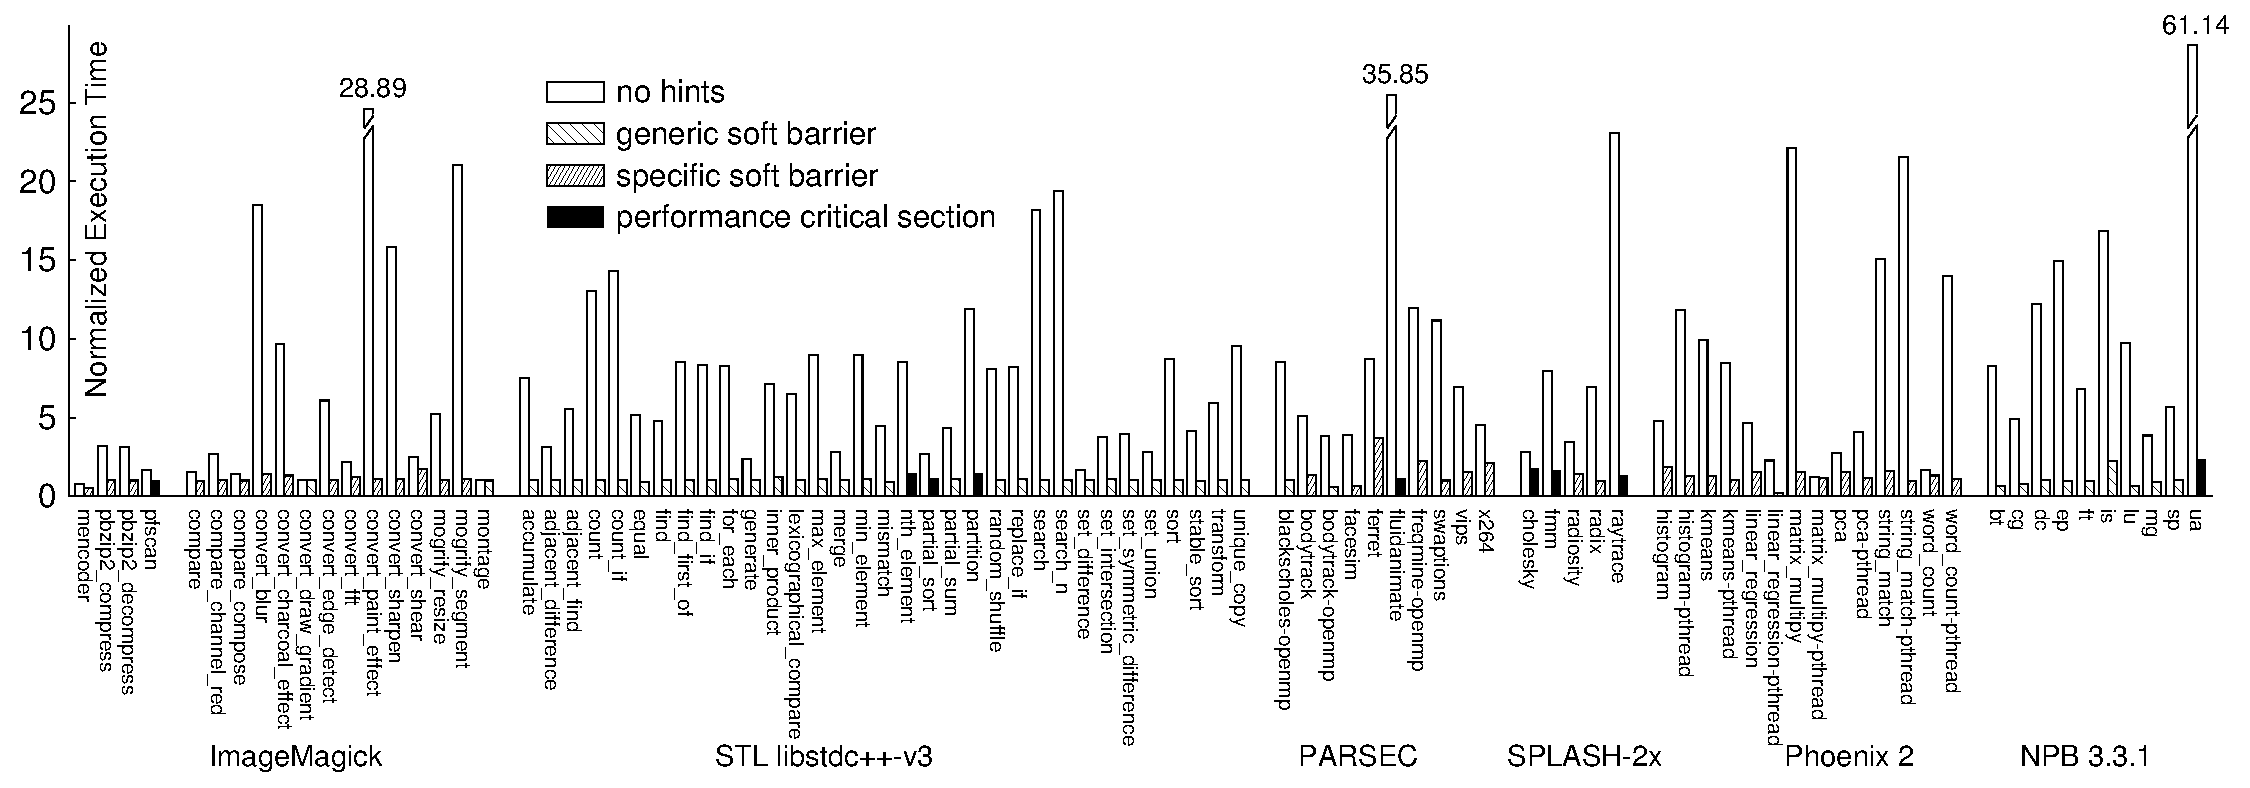
\includegraphics[width=0.57\textwidth]{parrot/figures/hints}
\vspace{-.20in}
\caption{{\em Effects of performance hints.} They reduced \parrot's overhead from \overallnohints to \overallhints.} \label{fig:parrot-overhead-hints}
\vspace{-.05in}
\end{figure*}

\begin{table}[!hb]
\footnotesize
\centering
\vspace{-.05in}
\begin{tabular}{lrr}
{\bf Program} & {\bf Success} & {\bf Timeout} \\
\hline
\convertshear                  & 725        & 1           \\
\bodytrack                        & 60,071   & 2,611     \\
\ferret                           & 699        & 2           \\
\vips                             & 3,311       & 6           \\
\xtwosixfour                             & 39,480      & 148,470      \\
\radiosity                      & 200,316     & 7,266        \\
\histogram                       & 167        & 1           \\
\kmeans                          & 1,470       & 196         \\
\pca                             & 119        & 2           \\
\pcapthread                     & 84         & 1           \\
\stringmatch                   & 64         & 1           \\
\wordcnt                     & 15,468      & 11          \\
\end{tabular}
\vspace{-.05in}
\caption{{\em \Compute successes and timeouts.}} \label{tab:parrot-timeouts}
\end{table}

Figure~\ref{fig:parrot-overhead-hints} compares \parrot's performance with and
without hints.  For all the \nprogneedhints programs that 
have hints, their mean overhead was reduced from
\overallnohints to \overallhints after hints were added. The four lines of generic
\compute hints in \libgomp (Table~\ref{tab:parrot-computehints}) 
reduced the mean overhead from \genericnolineup
to \genericlineup for \nproggenericlineuphints programs, program-specific
\computes from \specificnolineup to \specificlineup for
\nprogspecificlineuphints programs, and \nondets from \nondetnohints
to \nondethints for 9 programs.  \Computes timed out on
\nlineupfails programs (Table~\ref{tab:parrot-timeouts}), which affected neither
determinism nor correctness. The  \kmeans experienced over 10\% timeouts,
causing higher overhead. \xtwosixfour experienced many timeouts
but enjoyed partial coscheduling benefits (\S\ref{sec:parrot-hints}).

%% Table~\ref{tab:timeouts} shows that \nlineupfails programs had \compute
%% timeouts over all \nproglineuphints programs that requried \compute hints.
%% The reason of timeouts is that the workload of a program may not be evenly
%% divided by the number of threads, so some threads may handle more
%% computation than others.  Therefore, the \compute hints are suitable to
%% \parrot runtime rather than tranditional \pthread barrier, which may corrupt
%% program logic. Even timeout happened, these hints could still largely
%% speed up programs (Figure~\ref{fig:overhead-hints}).

%% generic: 6.6 times to 2.4\%, 41 programs
%% specific: 7.5 times to 33.9\%, 34 programs
%% nondet: 17.5 times to 49\%, 9 programs
%% all: 8 times to 19.6\%, 84 programs

%% First, even most of programs got 24 threads and all of them got 16+ threads, 
%% the overall overhead is still very reasonable.

%% For real applications, the overhead is negligble, and for benchmarks they are modist (recall that
%% our benchmarks are complete, and strictly run largest standard workloads, compared to other systems).

%% Second, mention the "effects of performance hints" here, ask yi-hong to provide 
%% the mean speedup XXX, which shows our hints are powerful.

%% Some programs such as mplayer and xx have significant speedup because in mplayer we saved
%% context switches (Hao provides concrete results here) and xx has better cpu affinity (by our
%% hybrid wait, yihong has studied this program).

%% Some program such as parsec mapreduce still have some siginificant amout of overhead (around 50\%)
%% because the workload is not evenly divided, so we pay some dynamic load imbalance here.

\subsection{Comparison to Prior Systems} \label{sec:parrot-comparison}

We compared \parrot's performance to \dthreads and \coredet.  We configured
both to provide the same determinism guarantee as \parrot,\footnote{While
  \kendo's determinism guarantee is closest to \parrot's, we tried and failed
  to acquire its code.}  so their overhead measured only the overhead to
make synchronizations deterministic.  One caveat is that neither system is
specially optimized for this purpose.  We managed to make only
\nprogcompared programs work with both systems because not both of them
support programming constructs such as read-write locks, semaphores,
thread local storage, network operations, and timeouts. These programs are
all benchmarks, not real-world programs.

Figure~\ref{fig:parrot-comparison} shows the comparison results.
\parrot's mean overhead is \parrotcompoverhead,
whereas \dthreads's is \dthreadssyncoverhead and \coredet's is
\coredetoverhead. 
%% When we turned on this protocol, we observed \dthreadsoverhead overhead.
\dthreads's overhead is mainly from serializing
parallel computations. \dedup, \ferret, \fluidanimate, 
\barnes, \radiosity, and \raytrace have over 500\%
overhead.  \fluidanimate is the slowest, whose threads wasted 59.3\% of their time
waiting for the other threads to do synchronizations.
%% both the internal fence (59.3\% of all threads' exeuction time) and the serialization
%% of synchronization operations (11.3\%) after the fence in \dthreads implementation.
Without \fluidanimate, \dthreads's overhead is still
\dthreadssyncoverheadnoflui.  (Performance hints may also help
\dthreads mitigate the serialization problem.)  \coredet's overhead is
mainly from counting instructions. \ferret, \fluidanimate, \barnes, and
\raytrace have over 300\% overhead.

\begin{figure}[t]
\centering
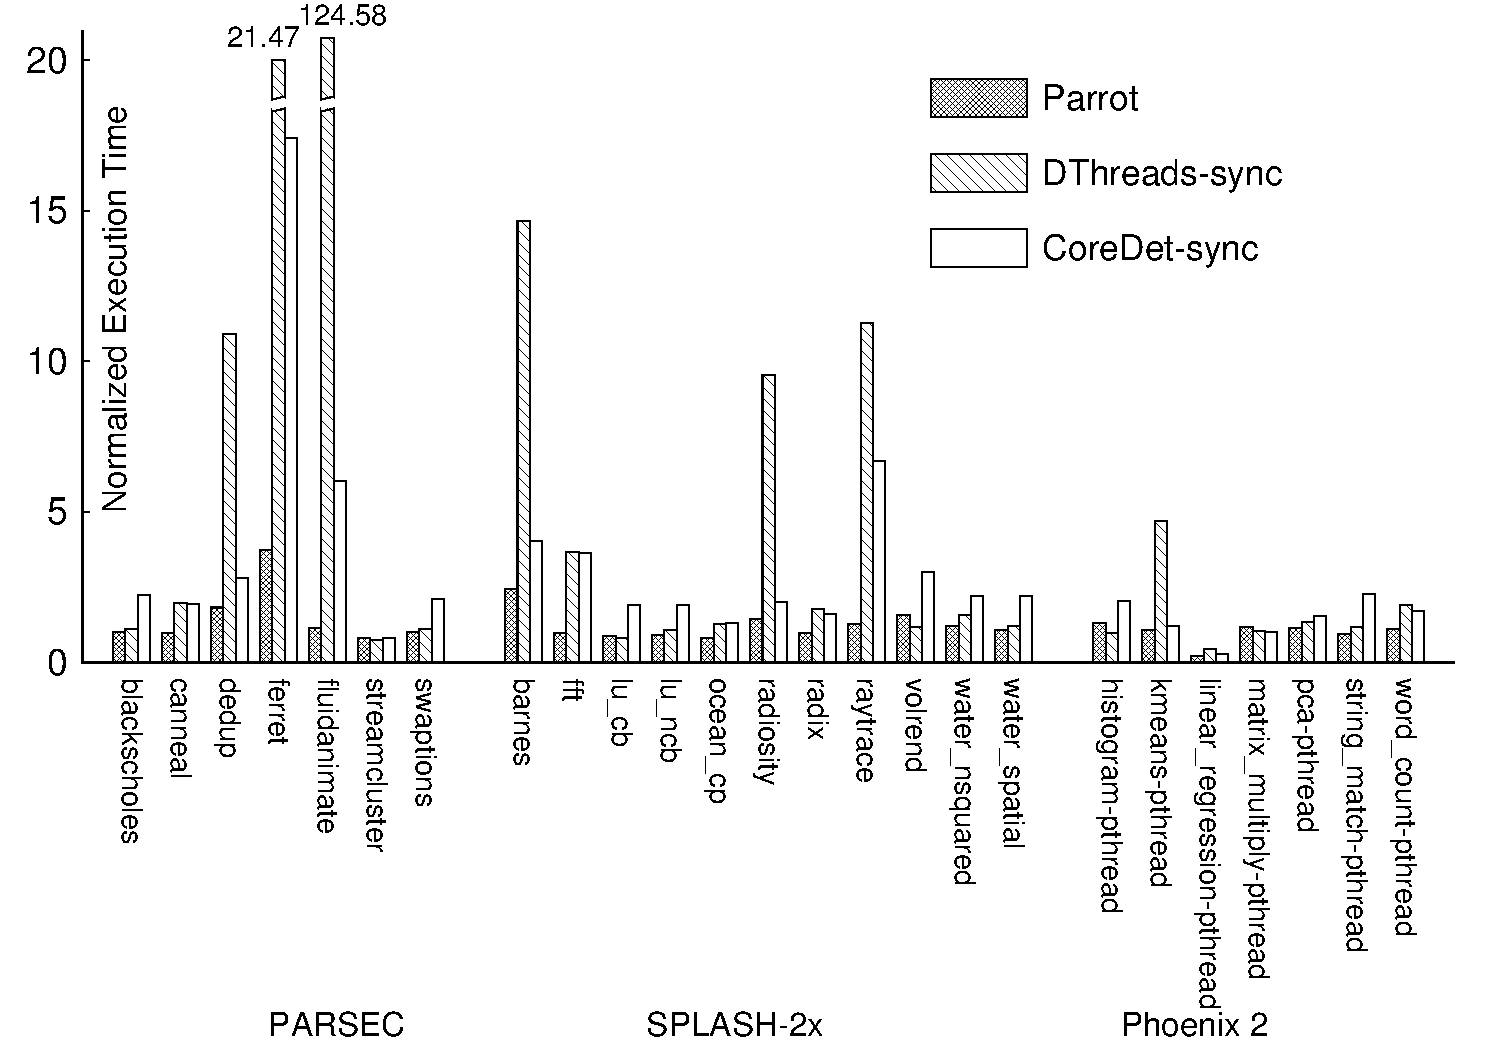
\includegraphics[width=0.57\textwidth]{parrot/figures/comparison}
\vspace{-.2in}
\caption{{\em \parrot, \dthreads, and \coredet overhead.}} \label{fig:parrot-comparison}
\vspace{-.0in}
\end{figure}

%% Note that 
%% our evaluation had more programs, (mostly) larger 
%% inputs, and more threads than the previous 
%% evaluations of the two systems. We did reduce these 
%% evaluation scales to be similar as theirs and observed 
%% compatible results as they reported.

%% First, we could run much more programs than prior systems, while the \dthreads
%% and \coredet could not run any of the real applications we have, based on the 
%% limitations (yi-hong has summarized them on a wiki page) we found.

%% Must mentioned that what modifications we changed (without affecting program 
%% logics) in those programs (such as killing shared stack objects) and made these 
%% programs work with both the other two (ask yi-hong for the modifications we made).

%% For the 30+ programs that can run with both the other two systems, we compared 
%% performance over standard largest workload and same thread settings, their 
%% overhead are \overdthreadsfull and \overcoredet times bigger than us (ask yi-hong 
%% for the mean overhead of the three systems, including ours).

%% parrot: consistently smaller
%% parrot: 79.5\%
%% dthreads: 31.9x, serialization on fluidanimate, histogram, kmeans, word\_count > 50x
%% coredet: 5.2x, string\_match-pthreads, kmeans, work\_count, string\_match > 15x

%% \begin{table}
%% \begin{tabular}{l|r}
%% {\bf System} & {\bf \# Supported} \\
%% \coredet   &  27 $\rightarrow$ 35 \\
%% \dthreads  &  24 $\rightarrow$ 31 \\
%% \parrot       & \nprog \\
%% \end{tabular}
%% \caption{{\em Number of programs supported.} The first number is the
%%   number of programs originally supported by the system, and the second
%%   after we tried our best to modify the evaluated programs to make them
%%   work with the system.}
%% \end{table}

\subsection{Scalability and Sensitivity} \label{sec:parrot-sensitivity}

%% Uncomment for the journal version of this paper

%% \begin{figure}[t]
%% \centering
%% 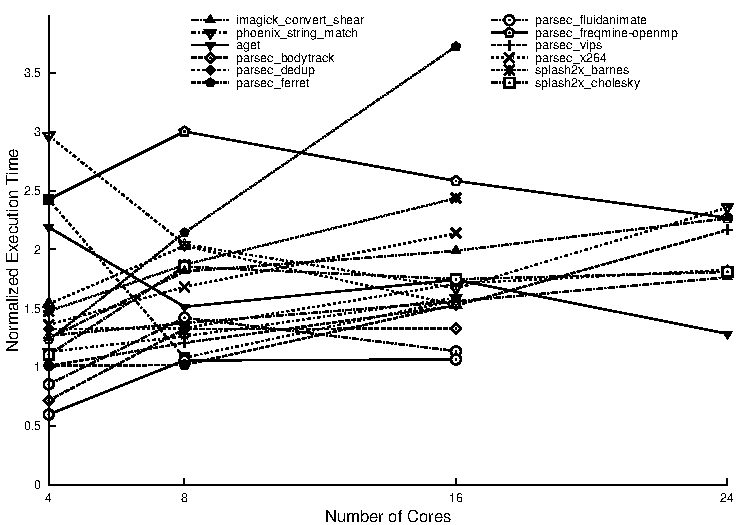
\includegraphics[width=\columnwidth]{figures/overhead_scalibility_bug}
%% \caption{{\em \parrot's scalability to the number of cores.} Legend lists
%%   only programs with over 25.0\% variance; the other programs are shown as
%%   light gray lines.} \label{fig:scalability}
%% \end{figure}

%% \begin{figure}[t]
%% \centering
%% 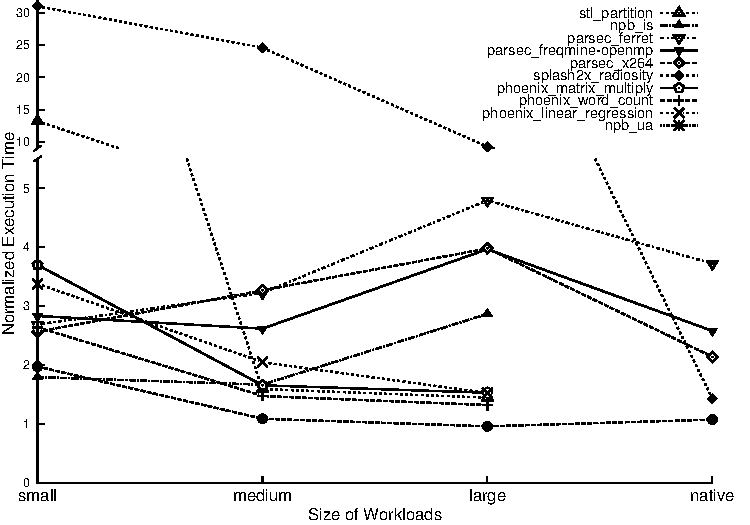
\includegraphics[width=\columnwidth]{figures/workload_sensitivity}
%% \caption{{\em \parrot's scalability to workloads.}  Legend lists only
%%   programs with over 60.0\% variance; the other programs are shown as
%%   light gray lines.} \label{fig:workloads}
%% \end{figure}
%% %% the variance is around 50%

%% Figure~\ref{fig:scalability} shows \parrot's scalability on our 24-core
%% machine. The overhead of most programs varies less than 25.0\% (light gray lines).
%% The overhead of other programs varies more, but stays below 2$\times$
%% except \ferret.  It scales worst because it uses pipeline and more threads
%% lead to more \compute timeouts during pipeline startup and teardown.

%% Figure~\ref{fig:workloads} shows \parrot's scalability on three or four
%% different scales of workloads defined by the benchmark authors.
%% The overhead of most programs varies less than 60.0\% (light gray
%% lines).  The \partition and \radiosity programs have large
%% overhead on smaller workloads because the workloads run too short.  For
%% instance, \v{radiosity}'s native workload runs for over 200s, but its
%% large workload runs for less than 3s and medium and small workloads
%% for less than 0.4s.  We also tried \redis on 15 different types of
%% workloads, and \mencoder on 5.  The results are similar to what we have
%% shown.  To summarize, the performance of \parrot and its hints are robust
%% to core counts, workload scales, and workload types.

We measured \parrot's scalability on our 24-core machine. All programs
varied within 40.0\% from each program's mean overhead across different core counts
except \ferret (57.4\%), \vips (46.7\%), \volrend (43.1\%), and
\linearregrepthread (57.1\%).  Some of these four programs use pipelines, so more
threads lead to more \compute timeouts during pipeline startup and
teardown.  We also measured \parrot's scalability on three or four different
workload scales as defined by the benchmark authors.  All programs
varied within 60\% from each program's mean overhead across different scales except
14 programs, of which 9 varied from 60\%--100\%, 3 from 100\%--150\%, and
2 above 150\%.  The 2 programs, \partition and \radiosity, went above
150\% because their smaller workloads run too short. For instance,
\v{radiosity}'s native workload runs for over 200s, but its large workload
runs for less than 3s and medium and small workloads for less than 0.4s.
We also ran \redis on 15 types of workloads, and \mencoder on
5.  The overhead did not vary much.  To summarize, \parrot's performance is
robust to core count and workload scale/type. (See~\cite{Parrot:github}
for detailed scalability results.)



\subsection{Determinism} \label{sec:parrot-determinism}

We evaluated \parrot's determinism by verifying that it computed the same
schedules given the same input.  For all programs except those with
\nondets, ad hoc synchronizations, and network operations, \parrot is
deterministic.  Our current way of marking ad hoc synchronization causes
nondeterminism; annotations~\cite{syncfinder:osdi10} can solve this
problem.  We also evaluated \parrot's determinism using a modified version of
\racey~\cite{racy-stress} that protects each shared memory access with a
lock.  In \racey, each different schedule leads to a different result with
high probability.  We executed our modified \racey 1,000 times without
\parrot, and saw 1,000 different results.  With \parrot, it always computed the
same result.

%% Evaluated the determinism of sync operations with \racey. Added the same
%% mutex lock to protect each shared memory access in source code, and then
%% run both non-det (original) executions and executions with \parrot, both with
%% 1000 times. For non-det executions, each run shows different hash
%% results. For executions with xxx, each run shows same results. This shows
%% that our locks are scheduled deterministically.

\subsection{Model Checking Coverage} \label{sec:parrot-coverage}

\begin{table}[!ht]
\footnotesize
\centering
\begin{tabular}{ccl}
{\bf Bin } & {\bf \# of Programs} & {\bf State Space Size with \dbug} \\
\hline
A & 27 & $1$ $\sim$ $14$ \\
B & 18 & $28$ $\sim$ $47,330$ \\
C & 25 & $3.99\times10^{6}$ $\sim$ $1.06\times10^{473}$ \\
D & 25 & $4.75\times10^{511}$ $\sim$ $2.10\times10^{19734}$ \\
%E & 1 & N/A \\
\end{tabular}
\vspace{-.05in}
\caption{{\em Estimated \dbug's state space sizes on programs with no
    \nondet nor network operation.}  } \label{tab:parrot-state-space-compute}
\vspace{-.05in}
\end{table}

\begin{table}[!hb]
\footnotesize
\centering
\vspace{-.05in}
\begin{tabular}{lrrr}
{\bf Program} & {\bf \dbug} & {\bf \ecosys} & {\bf Time} \\
\hline\\[-2.3ex]
%% redis smt+mc results not out yet.
%% redis                                    & $1.40\times10^{178}$    & N/A   & No       \\
\openldap                       & $2.40\times10^{2795}$        & $5.70\times10^{1048}$    & No        \\
\redis                       & $1.26\times10^{8}$        & $9.11\times10^{7}$    & No        \\
\pfscan                                   & $2.43\times10^{2117}$     & $32,268$   & $1,201$s     \\
\aget                       & $2.05\times10^{17}$        & $5.11\times10^{10}$    & No        \\
\nthelement                        & $1.35\times10^{7}$     & $8,224$   & $309$s      \\
\partialsort                       & $1.37\times10^{7}$     & $8,194$   & $307$s      \\
\partition                           & $1.37\times10^{7}$     & $8,194$   & $307$s      \\
\fluidanimate                     & $2.72\times10^{218}$        & $2.64\times10^{218}$  & No        \\
\cholesky                       & $1.81\times10^{371}$      & $5.99\times10^{152}$   & No   \\
\fmm                           & $1.25\times10^{78}$       & $2.14\times10^{54}$   & No        \\
\raytrace                       & $1.08\times10^{13863}$        &  $3.68\times10^{13755}$   & No        \\
%% UA smt+mc results not out yet.
%%\ua                                  & $>$ \v{DBL\_MAX}        & $>$ \v{DBL\_MAX}   & No        \\
\end{tabular}
\vspace{-.05in}
\caption{{\em Estimated state space sizes for programs containing
    \nondets.}  \ecosys finished 4 real-world programs (time in
  last column), and \dbug none.} \label{tab:parrot-state-space-nondet}
\end{table}

%% We formed an \ecosys by integrating \parrot with \dbug. Within 
%% this \ecosys, \parrot determinsitically schedules all \pthread synchronizations 
%% for \dbug except those in \nondet, and \dbug systematically explores 
%% all possible schedules of network events and operations within 
%% \nondet for \parrot. But forming this \ecosys, we expect that 
%% \parrot should drastically reduce the state space of a program and
%% increase testing coverage for \dbug, and \dbug can focus on
%% exploring the schedules that matter to \parrot. We enabled 
%% dynamic partial order reduction when running both \ecosys and \dbug.
%% We focus on evaluating how well \parrot can improve 
%% testing coverage for \dbug and how effectively \dbug can explore 
%% the schedules that matter to \parrot in \ecosys.

%% because
%% checking them requires including both endpoints in the checked system
%% (\eg, to check \aget, we have to check it together with a web server). 

%% We excluded two programs \ua and \volrend, because they contain too
%% many (132M and 57M respectively) synchronization operations which
%% caused \dbug to run out of memory.

To evaluate coverage, we used small workloads and two threads per workload.
Otherwise, the time and space overhead of \dbug,
or model checking in general, becomes prohibitive. Consequently, \parrot's
reduction measured with small state spaces is a conservative estimate of
its potential.  Two programs, \volrend and \ua, were excluded because they
have too many synchronization operations (\eg, 132M for \ua), causing
\dbug to run out of memory.  Since model checking requires a closed
(no-input) system, we paired \aget with lightweight web server
\mongoose~\cite{mongoose}).  We enabled
state-of-the-art DPOR~\cite{flanagan:dynamicpo} to evaluate how much more
\parrot can reduce the state space. We checked each program for a maximum of
one day or until the checking session finished.  We then compared the
estimated state space sizes.




%% programs, and we ran both the client and server processes with \dbug and
%% \ecosys (for \aget, we setup a \mongoose server~\cite{mongoose}).


%% Three programs, \openldap, \redis, and \aget, are client or server
%% programs, and we ran both the client and server processes with \dbug and
%% \ecosys (for \aget, we setup a \mongoose server~\cite{mongoose}).


% Programs are divided  into four bins based on the estimated   sizes.

%% in one day. Sorted by state space and
%%   classified by every 15. Our EcoSystem can finish testing all of them
%%   using only one deterministic schedule, and \dbug can only finish testing
%%   12 of the last 14 programs.  Seven programs of the last 14 are fork-join
%%   programs and have only one schedule.

%% Note: do not need to mention five bins, because the title of the table has mentioned this.
%% Table~\ref{tab:state-space-compute} shows all programs 
%% that need no hints or only \computes, divided into five bins based on state space size.

Table~\ref{tab:parrot-state-space-compute} bins all 95 programs that contain
(1) no network operations and (2) either no hints or only \computes. For each program,
\ecosys reduced the state space down to just one
schedule and finished in 2 seconds. \dbug alone could finish only
\nprogverifieddbug (out of 45 in bin A and B) within the time limit.
% The reduction for the bins C and D ranges from \shrinkscale.


Table~\ref{tab:parrot-state-space-nondet} shows the results for all
\nprognondetandnetwork programs containing network operations or
\nondets.  For all four real-world programs \pfscan, \partition,
\nthelement, and \partialsort, \ecosys effectively explored all
schedules in seven hours or less, providing a strong reliability
guarantee.  These results also demonstrate the power of \parrot:
the programs can use the checked schedules at runtime for speed.

To summarize, \parrot reduced the state space by \shrinkscale for
\nprogshrink programs (50 programs in Table~\ref{tab:parrot-state-space-compute},
6 in Table~\ref{tab:parrot-state-space-nondet}).  It increased the number of
verified programs from \nprogverifieddbug to \nprogverifiedxxx (95
programs in Table~\ref{tab:parrot-state-space-compute}, 4 in
Table~\ref{tab:parrot-state-space-nondet}).

%  These results also demonstrate the flexibility of \parrot: once schedules
%  are checked, \parrot can use the schedules at runtime for better
%  performance.

%{\bf TODO:} Add \ua and discuss \raytrace.

%% results are promising because \parrot can safely ignore these operations in
%% \nondet and run with these programs with reasonable overhead. For the five
%% benchmark programs \fluidanimate, \cholesky, \fmm, \raytrace and \ua,
%% \ecosys could not finish exploring their state space within one day. Maybe
%% combining \ecosys with some other more effectively reduction techniques
%% could solve this problem.  Nontheless, normally people may care about
%% correctness of real applications over benchmark programs (For \redis,
%% currently we are working in progress on running it with \ecosys.).

%% Table~\ref{tab:computehints} shows all the 95 programs without 
%% \nondet hints. \ecosys can drastically reduce their huge state 
%% space to one fast (via our \compute hints) and deterministic 
%% schedule within few seconds, effectively improve testing coverage for these 
%% programs, while \dbug could only finish exploring  the schedules 
%% of 12 programs (seven of them are fork-join programs, six 
%% from phoenix, one from \parsec, and they 
%% only have one schedule) within one day run. For 81 out of 
%% the 95 programs, \ecosys proactively shrinks their state 
%% space by at least $10^{4}$, and 51 of these programs have a 
%% state space larger than $10^{10}$, so by comparing 
%% these state space with the number of schedules have been 
%% explored within one day, we estimated that the state space  
%% of these 51 programs could not be completely explored by 
%% \dbug within a few years.

%% Table~\ref{tab:nondethints} shows all the 10 programs that 
%% may contain nondeterministic events such as network or 
%% operations within \nondet. For four real applications \pfscan, 
%% \partition, \nthelement, and \partialsort, \ecosys can 
%% effectively explore all their schedules within seven hours, 
%% because \ecosys runs \parrot to deterministically schedule 
%% lots of \pthread synchronization operations and enables \dbug to 
%% focus on only exploring those schedules that matter to 
%% \parrot. We estimated that \dbug won't finish exploring 
%% scheduels for these four programs within a few years.
%% These results are promising because \parrot can 
%% safely ignore these operations in \nondet and run with 
%% these programs with reasonable overhead. For the five benchmark 
%% programs \fluidanimate, \cholesky, \fmm, \raytrace and \ua,
%% \ecosys could not finish exploring their state space within 
%% one day. Maybe combining \ecosys with some other more 
%% effectively reduction techniques could solve this problem. 
%% Nontheless, normally people may care about correctness of real applications
%% over benchmark programs (For \redis, currently we are working in progress on 
%% running it with \ecosys.).



\vspace{-.02in}
\section{Related Work} \label{sec:parrot-related}
\vspace{-.02in}

\para{DMT and \smt systems.}  Conceptually, prior
work~\cite{dthreads:sosp11, cui:tern:osdi10, peregrine:sosp11,
  determinator:osdi10}, including ours~\cite{cui:tern:osdi10,
  peregrine:sosp11}, conflated determinism and stability.  To our
knowledge, we are the first to distinguish these two separate
properties~\cite{smt:cacm,smt:hotpar13}.

Implementation-wise, several prior systems are not backward-compatible
because they require new hardware~\cite{dmp:asplos09}, new
language~\cite{dpj:oopsla09}, or new programming model and
OS~\cite{determinator:osdi10}.  Among backward-compatible systems, some
DMT systems, including \kendo~\cite{kendo:asplos09},
\coredet~\cite{coredet:asplos10}, and \coredet-related
systems~\cite{dos:osdi10, ddos:asplos13}, improve performance by balancing
each thread's load with low-level instruction counts, so they are not
stable.

Five systems can be classified as \smt systems.  Our
\tern~\cite{cui:tern:osdi10} and \peregrine~\cite{peregrine:sosp11} systems
require sophisticated program analysis to determine input and schedule
compatibility, complicating deployment. Bergan {\it et
  al}~\cite{bergan:oopsla13} built upon the ideas in \tern and \peregrine
to statically compute a small set of schedules covering all inputs, an
undecidable problem in general.  \grace~\cite{grace:oopsla09} and \dthreads~\cite{dthreads:sosp11} ignore thread load
imbalance, so they are prone to the serialization problem
($\S$\ref{sec:parrot-example}). \grace also requires
fork-join parallelism.

Compared to \parrot's evaluation, prior evaluations have several limitations.
First, prior work has reported results on a narrow set of programs,
typically less than 15.  The programs are mostly synthetic benchmarks, not
real-world programs, from incomplete suites.  Second, the experimental
setups are limited, often with one workload per program and up to 8
cores.\footnote{Three exceptions used more than 8 cores:
  \cite{kendo:wodet11} (ran a 12-line program on 48 cores),
  \cite{aviram:thesis} (ran 9 selected programs from \parsec, \splashx, and
  \npb on 32 cores), and \cite{dmp:asplos09} (emulated 16 cores).}

Lastly, little prior work except ours~\cite{wu:pldi12} has demonstrated how the
approaches benefit testing or reported any quantitative results on
improving reliability, making it difficult for potential adopters to
justify the overhead.

\para{State-space reduction.} \parrot greatly reduces the state space of
model checking, so it bears similarity to \emph{state-space reduction
  techniques} (\eg,~\cite{godefroid:verisoft, flanagan:dynamicpo,
  demeter:sosp11}).  Partial order
reduction~\cite{godefroid:verisoft, flanagan:dynamicpo} has been the main
reduction technique for model checkers that check implementations
directly~\cite{modist:nsdi09, dbug:spin11}.  It detects
permutations of independent events, and checks only one permutation
because all should lead to the same behavior.  Recently, we proposed
dynamic interface reduction~\cite{demeter:sosp11} that checks loosely
coupled components separately, avoiding expensive global exploration of
all components.  However, this technique has yet to be shown to work well
for tightly coupled components such as threads communicating
via synchronizations and shared memory.
% (The explorer of each component in~\cite{demeter:sosp11} has to explore
% many different schedules, which \parrot can help reduce.)

\parrot offers three advantages over reduction techniques
(\S\ref{sec:parrot-mc}): (1) it is much simpler because it does not
need equivalence to reduce state space; (2) it remains effective as the
checked system scales; and (3) it works transparently to reduction
techniques, so it can be combined with them for further reduction.  The
disadvantage is that \parrot has runtime overhead.

\para{Concurrency.} Automatic mutual exclusion (AME)~\cite{ame:hotos07} assumes all shared
memory is implicitly protected and allows advanced developers the
flexibility to remove protection.  It thus shares a similar high-level
philosophy with \parrot, but the differences are obvious.  We are unaware of
any publication describing a fully implemented AME system. \parrot is
orthogonal to much prior work on concurrency error
detection~\cite{yu:racetrack:sosp,savage:eraser,racerx:sosp03,lu:muvi:sosp,avio:asplos06,conmem:asplos10},
diagnosis~\cite{racefuzzer:pldi08,ctrigger:asplos09,atomfuzzer:fse08}, and
correction~\cite{dimmunix:osdi08,gadara:osdi08,wu:loom:osdi10,cfix:osdi12}. By
reducing schedules, it potentially benefits all these techniques.

\vspace{-.05in}
\section{Summary} \label{sec:tern-summary}
\vspace{-.05in}

We have presented \parrot, a simple, practical \pthread-compatible system for
making threads deterministic and stable. It offers a new contract to
developers.  By default, it schedules synchronizations using round-robin,
vastly reducing schedules.  When the default schedules are slow, it
allows developers to write performance hints for speed.  We believe this
contract eases writing correct, efficient programs.  We have
also presented an ecosystem formed by integrating \parrot with model checker
\dbug, so that \dbug can thoroughly check \parrot's schedules, and \parrot can
greatly improve \dbug's coverage.  Results on a diverse set of \nprog
programs, roughly \overeach more than any prior evaluation,
show that \parrot is easy to use, fast, and scalable; and it improves \dbug's
coverage by many orders of magnitude.  We have released \parrot's source
code, entire benchmark suite, and raw results at \github.


